% !TEX root = A0_thesis_detecting_collusion_corruption_fraud.tex
\chapter{The World Bank's Procurements}\label{chap_procurements}

As shown in the chapter \ref{chap_intro}, The World Bank Group provides Financial Products and Services by giving out low-interest loans, zero to low-interest credits, and grants to developing countries. They offer financing through trust fund partnerships with bilateral and multilateral donors.  This work focuses in these Financial Products and Services. It analyzes their contracts by using historical data on over 300,000 major contracts funded by World Bank.

In this chapter BLA BLA BLA...BLA BLA

\section{The Wold Bank Group's Rules and Guidelines}

The process by which the World Bank Group gives out low-interest loans, zero to low-interest credits, and grants to developing countries is not simple. They have a set of guidelines, available online \parencite{wb_g_proc}, in which they specify how to apply to all the contracts for goods, works and services financed in whole or in part from the Bank's loans, credits and grants which would thereby cover both International Bank for Reconstruction and Development (IBRD) and the International Development Association (IDA). Similar provisions apply for the selection of Consultants under the Consultants Guidelines \parencite{wb_g_cons}. For the purpose of this project the Consultants will not be deeply explained. 

In the World Bank's rules and guidelines they consider ``goods'' and ``works'' all the related services such as transportation, insurance, installation, commissioning, training, and initial maintenance. Also,  ``goods'' includes commodities, raw material, machinery, equipment, vehicles, and industrial plant. 

\begin{quote}
``This requirement is made applicable in each operation through the loan, credit or grant agreement thus making their use a legal obligation on the part of the Borrower. It applies as well to counterpart funds that are also used to finance contracts with loan/credit proceeds. In addition, parts of Bank-financed projects that are co-financed by other donors are also subject to Bank rules. This could also be the case under parallel financing when co-financiers agree to using Bank guidelines (leverage effect).''\parencite{wb_rules}
\end{quote}

In order to ensure that these legal provisions are observed during project implementation, Bank staff review and provide a ``no objection'' before the Borrower implements certain procurement decisions\footnote{For all International Competitive Bidding (ICB) and other high-value, high-risk, and otherwise complex contracts}. Bank staff will review all the contracts that have not been subject to Prior Review so as to ensure that the Guidelines were applied as required. Where this is found not to be the case, the Bank applies various remedies including \textit{mis-procurement}, which in most instances requires cancellation and refund of the funds in question\footnote{Advertising requirements vary depending on whether Procurement is subject to International Competitive Bidding (ICB) or National Competitive Bidding(NCB).}.


\subsection{Procurements General Considerations}

In every Procurement the World Bank expect that the responsibility for the implementation of the project, and therefore for the award and administration of contracts under the project, rests with the Borrower. The Bank, is required ensure that the proceeds of any loan are used only for the purposes for which the loan was granted, with due attention to considerations of economy and efficiency and without regard to political or other non-economic influences or considerations. While in practice the specific procurement rules and procedures to be followed in the implementation of a project depend on the circumstances of the particular case, four considerations generally guide the Bank's requirements:
\begin{enumerate}[a)]
\item ``the need for economy and efficiency in the implementation of the project, including the procurement of the goods, works, and non-consulting services involved;
\item the Bank's interest in giving all eligible bidders from developed and developing countries the same information and equal opportunity to compete in providing goods, works, and non-consulting services financed by the Bank;
\item  the Bank's interest in encouraging the development of domestic contracting and manufacturing industries in the Borrowing country; and
\item the importance of transparency in the procurement process.''\footnote{See \cite{wb_g_proc}.}
\end{enumerate}


\subsection{Procurement Plan}

Any firm or person interested in a procurement has to submit a Procurement plan to the World Bank in which they specify general characteristics of the project such as the Bank’s approval date of the procurement plan, the date of general procurement notice and the period covered by the procurement plan. It has to include the details concerning the goods and works and non-consulting services required for the project such as the Prior Review Threshold, prequalification,  proposed procedures for CDD components, reference to (if any) project operational/procurement manual, any other special procurement arrangements, and a summary of the procurement packages planned during the first 18 months after project effectiveness. With regard to the consultants, it has to include a prior review threshold, short list comprising entirely of national consultants, any other special aelection Arrangements (including advance procurement and retroactive financing, if applicable or delete if not applicable), and consultancy assignments with selection methods and time Schedule. The appendix \ref{app_proc_plan} shows a sample procurement plan to be filled \parencite{wb_sample_proc}. 


The World Bank's guidelines for procurement of goods, works, and non-consulting services \parencite{wb_g_proc} establishes that open competition is the basis for efficient public procurement.  In their articles, they state that each Borrower shall select the most appropriate method for the specific procurement. They have to choose between International Competitive Bidding (ICB) or National Competitive Bidding (NCB). This means, in most cases, ICB, properly administered, and with the allowance for preferences for domestically manufactured goods and, where appropriate, for domestic contractors for works under prescribed conditions is the most appropriate method. The Bank requires its Borrowers to obtain goods, works, and non-consulting services through ICB open to eligible suppliers, service providers, and contractors\footnote{Section II of these Guidelines describes the procedures for ICB \parencite{wb_g_proc}.}.

In order to satisfy these requirements, any procurement needs to be transparent, competitive and legal according to the guidelines the World Bank established. Contractors providing goods and services on World Bank projects are typically hired through a competitive bidding process. The problem is that in practice, the Borrowers and Contractors tend not to fulfill those requirements. Occasionally, prospective contractors influence the competitive system by colluding with other contractors, bribing government officials, or otherwise manipulating the bidding process. These offenses have far-reaching effects on the price and quality of contract delivery.  There is a considerable amount of cases in which corruption, collusion and/or fraud takes place. The guidelines include some sections to address those problems. The World Bank is committed to detecting instances of collusion, corruption, and fraud in order to maximize its global impact.

\section{Corruption, Collusion and Fraud}\label{sec_intro_corruption}

The World Bank's guidelines for procurement of goods, works, and non-consulting services \parencite{wb_g_proc} establishes what's to be understood by corruption, collusion, fraud, coercion and obstruction. 

It is the Bank's policy to require that Borrowers\footnote{including beneficiaries of Bank loans.}, bidders, suppliers, contractors and their agents\footnote{whether declared or not.}, sub-contractors, sub-consultants, service providers or suppliers, and any personnel thereof, observe the highest standard of ethics during the procurement and execution of Bank-financed contracts. In pursuance of this policy, the Bank defines, the terms set forth below as follows\footnote{Definitions taken from \cite{wb_g_proc}. Updated to 2011.}:

\begin{definition}\label{def_corruption}
A \textit{corrupt practice} is the offering, giving, receiving, or soliciting, directly or indirectly, of anything of value to influence improperly the actions of another party.
\end{definition}

\begin{definition}\label{def_collusion}
A \textit{collusive practice} is an arrangement between two or more parties designed to achieve an improper purpose, including to influence improperly the actions of another party.
\end{definition}

\begin{definition}\label{def_fraud}
A \textit{fraudulent practice} is any act or omission, including a misrepresentation, that knowingly or recklessly misleads, or attempts to mislead, a party to obtain a financial or other benefit or to avoid an obligation.
\end{definition}

\begin{definition}\label{def_coersion}
A \textit{coercive practice} is impairing or harming, or threatening to impair or harm, directly or indirectly, any party or the property of the party to influence improperly the actions of a party.
\end{definition}

\begin{definition}\label{def_obstruction}
A \textit{obstructive practice} is deliberately destroying, falsifying, altering, or concealing of evidence material to the investigation or making false statements to investigators in order to materially impede a Bank investigation into allegations of a corrupt, fraudulent, coercive or collusive practice; and/or threatening, harassing or intimidating any party to prevent it from disclosing its knowledge of matters relevant to the investigation or from pursuing the investigation, or acts intended to materially impede the exercise of the Bank's inspection and audit rights.
\end{definition}

In its effort to avoid practices from definitions \ref{def_collusion} to \ref{def_obstruction}, the World Bank
will respond accordingly to each contract in question. 
The Bank will \textit{reject a proposal} for award if it determines that the bidder recommended for award, or any of its personnel has, directly or indirectly, engaged in corrupt, fraudulent, collusive, coercive, or obstructive practices in competing for the contract in question. 
The Bank will \textit{declare mis-procurement} and cancel the loan if it determines at any time that representatives of the Borrower engaged in  any corrupt, fraudulent, collusive, coercive, or obstructive practices during the procurement or the implementation of the contract. 
The Bank will \textit{sanction} a firm or individual, including by publicly declaring such firm or individual ineligible, either indefinitely or for a stated period of time to be awarded a Bank-financed contract; and to be a nominated sub-contractor of an otherwise eligible firm being awarded a Bank-financed contract.
The Bank will require that a clause be included to permit the Bank to inspect all accounts, records, and other documents relating to the submission of bids and contract performance, and to have them audited by auditors appointed by the Bank.

\subsection{Examples: What is Fraud and Corruption?}

An example of fraud according to the definition \ref{def_fraud}: \begin{quote}
``In a few years since its establishment, a consulting company is awarded multiple World Bank Group-financed contracts totaling in millions of dollars.  The proposals submitted by the consulting company contain numerous past project experiences and references that contribute to its success and eligibility.  However, a review of the consulting company's past project experiences reveal that the company has claimed the experiences of individual consultants as its own, as well as grossly exaggerated the value of the projects that it has undertaken.  Not only is the consulting company misrepresenting its qualifications and capacity, it is also cutting its subconsultants' contracts by half, but claiming the full amount on its invoices to the client.  The quality of the deliverables from this consulting company is highly questionable, which affects the project's overall developmental goals.''\parencite{wb_examples}
\end{quote}

An example of corruption according to the definition \ref{def_corruption}: \begin{quote}
``A supplier agrees to pay kickbacks to a senior government official through an agent it hires as a sub-consultant to perform business development and marketing services but without any deliverables.  This agent is connected to a senior government official who is demanding a commission from every bidder as the official has influence over the bid evaluation committee and can steer the award of the contract to any bidder willing to pay.  This supplier builds in the kickback amount as a percentage of the contract value, and pays for it from the funds it receives from the World Bank Group-financed project. Project financing costs are artificially inflated by these practices, and the supplier recovers costs by providing less expensive and lower quality goods.''\parencite{wb_examples}
\end{quote}

% Collusion
An example of collusion according to the definition \ref{def_collusion}: \begin{quote}
``A project official arranges to steer contracts on a World Bank Group-financed project to his own company and that of his relatives.  The project official not only tells his relatives' companies what prices to put in their bids, but also what particular technical specification to include.  The bids of companies that are not part of this inner circle are disqualified as being technically non-responsive, leaving the project official's and his relatives' companies as the lowest evaluated bidders on the different contracts.  Not only is the integrity of the procurement process compromised, but the winning bid prices are considerably higher than what would have been with genuine competitive bidding.''\parencite{wb_examples}
\end{quote}

% Coercion
An example of coercion according to the definition \ref{def_coersion}: \begin{quote}
``A contractor is stopped from submitting his bid at the bid opening.  Persons connected to a competitor block the contractor from entering the building where the bid opening is taking place, and tell him that `if he cares for his family, he should not submit a bid.'  Another bidder who comes to submit a bid is also stopped by these same persons who tells the bidder that `it is not his turn to win this contract.'  The two bidders leave the bid opening and do not submit a bid out of fear.''\parencite{wb_examples}
\end{quote}

% Obstruction

An example of coercion according to the definition \ref{def_coersion}: \begin{quote}
``World Bank Group investigators contact a company alleged to have paid a bribe on a World Bank Group-financed contract and request to audit the company's financial records.  The company refuses to do so despite its agreement and obligation under the contract to allow the World Bank Group access to these records.  Furthermore, it withholds key documents and alters other documents that are given to the investigators.''\parencite{wb_examples}
\end{quote}


\section{World Bank Listing of Ineligible Contractors}

The World Bank has a long history of giving loans for procurement of goods, works, and non-consulting services based on the four considerations listed above. As expected, there has been a long history of malicious activity in the procurement process. This is why The World Bank publishes a list of contractors which had been discovered to have a practice that lead to either a rejection, a mis-procurement, an obstructive practice or a sanction. This project refers to this list as the debarment data.

The World Bank publishes an online \parencite{wb_debarment} list that includes all the firms and individuals listed as ineligible to be awarded a World Bank-financed contract for the periods indicated because they have been sanctioned under the Bank's fraud and corruption policy as set in the Procurement Guidelines or the Consultant Guidelines.  Such sanction was imposed as the result of an administrative process conducted by the Bank that permitted the accused firms and individuals to respond to the allegations\footnote{``Through July 2007, this process was conducted in accordance with the Sanctions Committee Procedures adopted on August 2, 2001. Since then, the process has been conducted in accordance with the Sanctions Procedures of the World Bank Group Sanctions Board.''}, or a cross-debarment\footnote{ Since 2011.} made effective by the World Bank, Asian Development Bank, European Bank for Reconstruction and Development, Inter-American Development Bank, and African Development Bank.

The table \ref{tab_debarred_sam} bellow shows a short sample of how is the debarments list published. As it can be seen from the table \ref{tab_debarred_sam}, it includes a \textit{Firm Name, Address, Country, Ineligibility Period} and \textit{Grounds}. The \textit{Firm Name} can be a person or an entity, the \textit{Ineligibility period} corresponds to the time frame in which that specific \textit{Firm Name} is debarred from receiving any type of award financed by the World Bank, and finally, the \textit{Grounds} refers to the violations made to the Consultants Guidelines (CG) or the Procurements Guidelines (PG) and their specific article and section.

\begin{table}[H]
\caption{Debarred Firms and Individuals (sample)}
\label{tab_debarred_sam}
\resizebox{\textwidth}{!}{
\begin{tabular}{lrrccr}
\hline
\hline
\multirow{2}{*}{Firm Name} & 	\multirow{2}{*}{Address} & \multirow{2}{*}{Country}	& \multicolumn{2}{c}{Ineligibility Period} & \multirow{2}{*}{Grounds} \\ \cline{4-5}
 & & & From & To & \\
\hline
MR. NGUYEN & TOWER CENTER  & Vietnam& 15-DEC-2015 &	14-DEC-2026	& CG, 1.22(a)(ii); PG, 1.14(a)(ii)-(iii) \\
 PHUONG & OFFICE   &  &  & &\\
 QUY*298 &BUILDING,NO.  &  & & & \\
 &83A LY THUONG  &  & & & \\
 &KIET  &  &  & &\\
 &STREET,DISTRICT & &  &  & \\
 &HOAN KIEM,  HANOI & & &  & \\

SFC VIETNAM  & TOWER CENTER & Vietnam & 15-DEC-2015	& 14-DEC-2025 &	CG, 1.22(a)(ii); PG, 1.14(a)(ii)-(iii) \\
INVESTMENT & OFFICE  &  &  & &\\
DEVELOPMENT & BUILDING, NO.  &  &  & &\\
FOR ENVIRONMENT& 83A LY THUONG  &  &  & &\\
CORPORATION*297& KIET STREET,  &  &  & &\\
& DISTRICT HOAN  &  &  & &\\
& KIEM,  HANOI	 &  &  & & \\

MR. NIKOLAI & ANTONIENKO 3,-43,	& Russian & 	30-OCT-2015	& 29-OCT-2019	& CG, 1.22(a)(i) \\
GEORGIEVITCH  &  190000 SAINT  &  Federation &  & &\\
OBRADOVITCH*296 & PETERSBURG    &  &  & &\\
\hline
\hline
\end{tabular}
}
\footnotesize{\textbf{Source:} see the \cite{wb_debarment}.\\ \textbf{Notes:} Several firms above are marked with an asterisk (*). The period of ineligibility of the sanctioned firm extends to any firm directly or indirectly controlled by the sanctioned firm.}
\end{table}


The World Bank also publishes a second list that includes the \textit{Other Sanctions} that includes firms that are typically under a \textit{Conditional Non-debarment}. ``The Conditional Non-debarment means that so long as the sanctioned entity meets certain conditions, including (a) implementing a corporate compliance program acceptable to the Bank; (b) fully cooperating with the Bank; and (c) not attempting to evade the sanction imposed on the firm and those entities it directly or indirectly controls, the sanctioned entity will continue to be eligible to participate in Bank-financed activities.''\parencite{wb_debarment}; or has a \textit{Letter of Reprimand} by which the World Bank officially notifies the firm its sanction.


\section{Investigations}

The World Bank conducts some investigations to determine whether to sanction or not an entity within the procurement process. The investigations are primarily based upon the allegations they receive, so it is extremely important that those people who are involved in activities supported by World Bank Group funds take the initiative to report suspected fraud or corruption. By now, the World Bank has a basic way of conducting investigations regarding corruption, collusion, fraud, coercion and obstruction.  The \cite{wb_investigations} lists three types of investigations by which the Bank analyze the sanctionable practices. 


\begin{enumerate}[1.]
\item \textit{Complaint Intake}, where Integrity Vice Presidency (INT) performs an initial assessment of every complaint that it receives.  This assessment determines whether: the complaint relates to a sanctionable practice in World Bank Group-financed projects, the complaint has credibility and the matter is of sufficient gravity to warrant an investigation.  Complaints outside of INT's jurisdiction are redirected to other areas of the World Bank Group as appropriate.  Complaints that fall under INT's jurisdiction are investigated if they are determined to be of a higher priority.  When a complaint does not reach this threshold, INT works with Operational staff to address the issues raised.  In assigning priority, INT also considers the possible reputational risk to the World Bank Group, amount of funds involved and quality of the information or evidence in INT's possession. 

\item \textit{Investigation of Cases}, where, through investigations, INT ascertains whether firms and/or individuals have engaged in one of the World Bank Group's five sanctionable practices.  Since an INT investigation is administrative in nature, the standard of proof is akin to a ``balance of probabilities'' and therefore lower than the criminal standard of ``beyond a reasonable doubt.'' The World Bank Group, for that reason, has to prove that it is more likely than not that the alleged misconduct has occurred.  If INT finds sufficient evidence to prove the allegation, the allegation is considered substantiated.  The allegation is considered unsubstantiated if there was insufficient evidence to prove or disprove it, and unfounded if the allegation has no basis in fact.

\item \textit{Investigation Reports}, when INT substantiates a case, it produces a Final Investigation Report (FIR).  In some cases, INT will produce an FIR even if there is not reasonably sufficient evidence to substantiate a complaint - for example, if INT believes that the investigation unearthed important lessons that should be shared with colleagues in the World Bank Group.  FIRs are sent to regional management for comment before being finalized and provided to the World Bank Group President. INT strives to ensure that the maximum time between opening a case and completing an investigation report is twelve months for normal cases and eighteen months for complex cases. FIRs also form the basis for two other INT outputs: referral reports, which INT sends to relevant national authorities if evidence indicates that the laws of a World Bank Group member country may have been violated; and redacted reports, which are provided to the World Bank Group's Board of Executive Directors and, after the completion of any related sanctions proceedings, posted on this site.
\end{enumerate}

\subsection{Report Suspected Fraud or Corruption}

The World Bank's Integrity Vice Presidency (INT) is in charge of taking care of any allegation that involves possible fraud, corruption, collusion, coercion and obstruction in World Bank-funded projects and/or against World Bank staff. To Report an allegation, the World Bank provides two main options, submit an Online Integrity Complaint Form or download the free Integrity Application. 

The Integrity Complaint Form is a way to send a report to INT. The figure \ref{fig_complaint} bellow shows the format of an Integrity Complaint Form. As the figure shows, it is a secure and confidential third-party website that is managed by INT. The form requires information regarding your allegations and a summary of the concerns. There's an option to upload supporting documents after submitting the Form.

\begin{figure}[H]
\caption{Integrity Complaint Form}
\label{fig_complaint}
\begin{center}
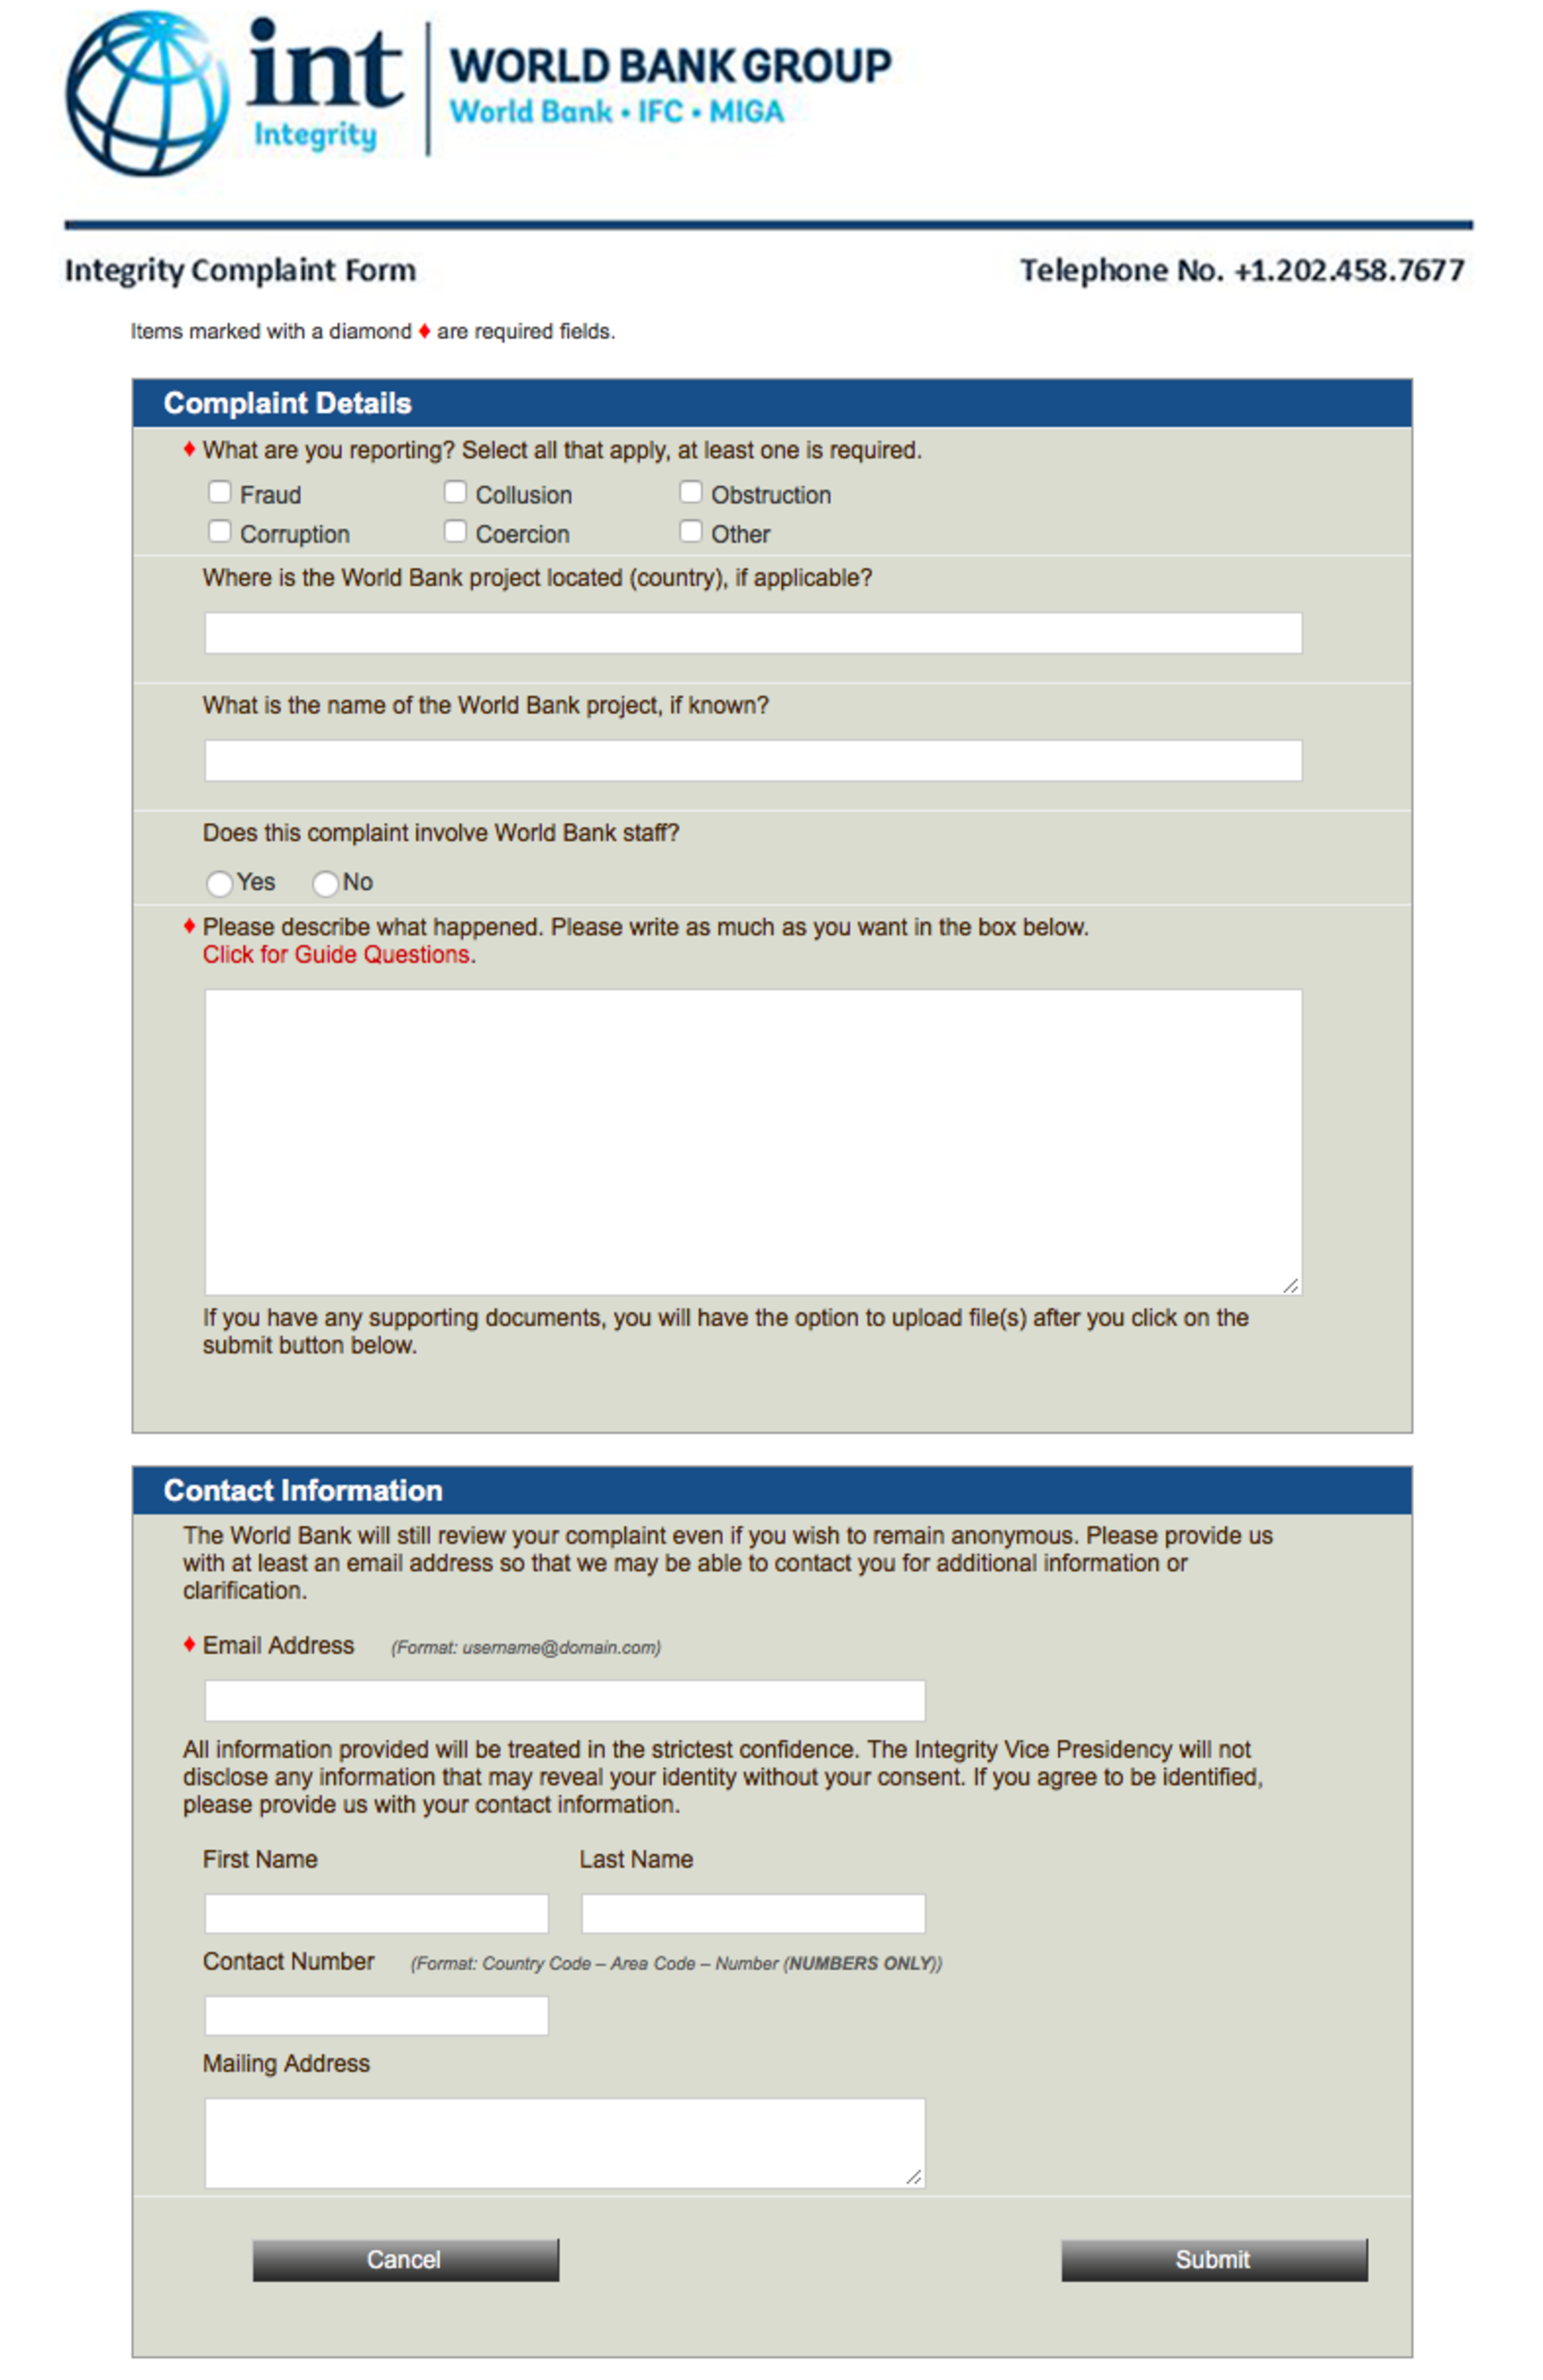
\includegraphics[max width=.75\textwidth]{../img/wb_report_complaint.pdf}
\end{center}
\noindent \footnotesize{\textbf{Source:} \cite{wb_complaint}}
\end{figure}


\section{Searching for \textit{red-flags} in data}

The real issue for the World Bank becomes that, in order for them to conduct a Complaint Intake, an Investigation Case, or even an Investigation Report, they rely on third parties. As seen in online form that the World Bank provides, figure  \ref{fig_complaint} and on the mobile application, they are making a significant effort to supply third parties with the best tools to report any cases of corruption, fraud, collusion, coercion and  obstruction so that reporting do not becomes the obstacle. Said that, the real problem for The World Bank becomes that their efforts to conduct investigations is limited to the information they receive from third parties. This is an important matter when their objective is to reduce the world poverty by awarding procurements, loans and credit to developing countries and at the same time they are facing corruption, fraud and collusion problems by which only few sectors are being benefited.

Investigators at the World Bank's Integrity Vice Presidency (INT) are responsible for investigating collusion, as well as the other sanctionable offenses of coercion, fraud and corruption in World Bank-financed projects. The challenge with a global portfolio is how to detect collusion or corruption, particularly if no one reports the incident.

For this reason, The World Banks has made an effort in order to conduct a new type of investigations that do not depend on third parties but depends on data. The problem now becomes: how to identify corruption, collusion, fraud, coercion and obstruction by looking on data? The World Bank has some initial thoughts and has been trying to search for new and innovative ways to tackle this problem. For example, on June 2014 they organized a DataSprint event that helped them to dive into data to address these type problems. The objective was to analyze, visualize, and mash-up the the data. I went to Washington, D.C. for several days of meetings and collaboration with the project partners at INT and the World Bank's Office of the Controller. The trip was an opportunity to learn what corruption, fraud, and collusion looks like in the data.

INT investigators have identified several patterns in bidding behavior that could point to collusion or other forms of corruption. Regular, periodic rotation of contract awards among a small group of contractors, for example, might indicate that bidders are working together to set prices or distribute contracts. Contractors may split large projects into multiple small ones, keeping individual contract values below a threshold that triggers additional review or competitive bidding. The total number of bidders shrinking over time might indicate that potential contractors are being pushed out of the market through some form of illegal coercion. While none of these findings represent clear-cut evidence of collusion, they are detectable clues that can help direct investigative efforts and ensure that the integrity of development is not compromised \parencite{dssg_proc}.

The INT developed a visualization, shown on figure \ref{fig_what_corr}, that show cases that suggest malicious practices. To start with, sub-figure \ref{fig_cum_value} shows data that corresponds to a case in which  six suppliers that are supposed to be competitive and all the cumulative value on non-competitive contracts are being assigned to suppler number one. On sub-figure \ref{fig_value} it is shown that contracts, that correspond to Company A, numbers one and two overcome the threshold for a common competitive biding. This might be suggesting collusion. Sub-figure \ref{fig_winning} shows a case where suppliers four to eight always bid a little less that the winning bid suggesting another type of collusion. Now, on sub-figure \ref{fig_month} there is a suggestion of favoritism that suggest corruption or even coercion in which the value of a non-competitive contract goes high exactly in the times of a governmental election. Sub-figure \ref{fig_links} suggests that companies that have contracts or directors in common with other companies that have been previously debarred are suspicious of malicious activities. As it can be seen from sub-figures 
\ref{fig_bid1} and \ref{fig_bid2} there tend to be bidding patterns in which take turns by bidding differently in each round such that they take turns to get the contracts. This affects directly the process making in non competitive. Lastly, it can be seen on figure \ref{fig_proposals} that as time pass, only two suppliers are the ones participating on proposals among a vast pool. This  fact is suggesting that those two suppliers might have done something  to coerce the others not to participate on proposals after time four.

\begin{figure}[H]
\begin{center}
\caption{What does corruption look like?}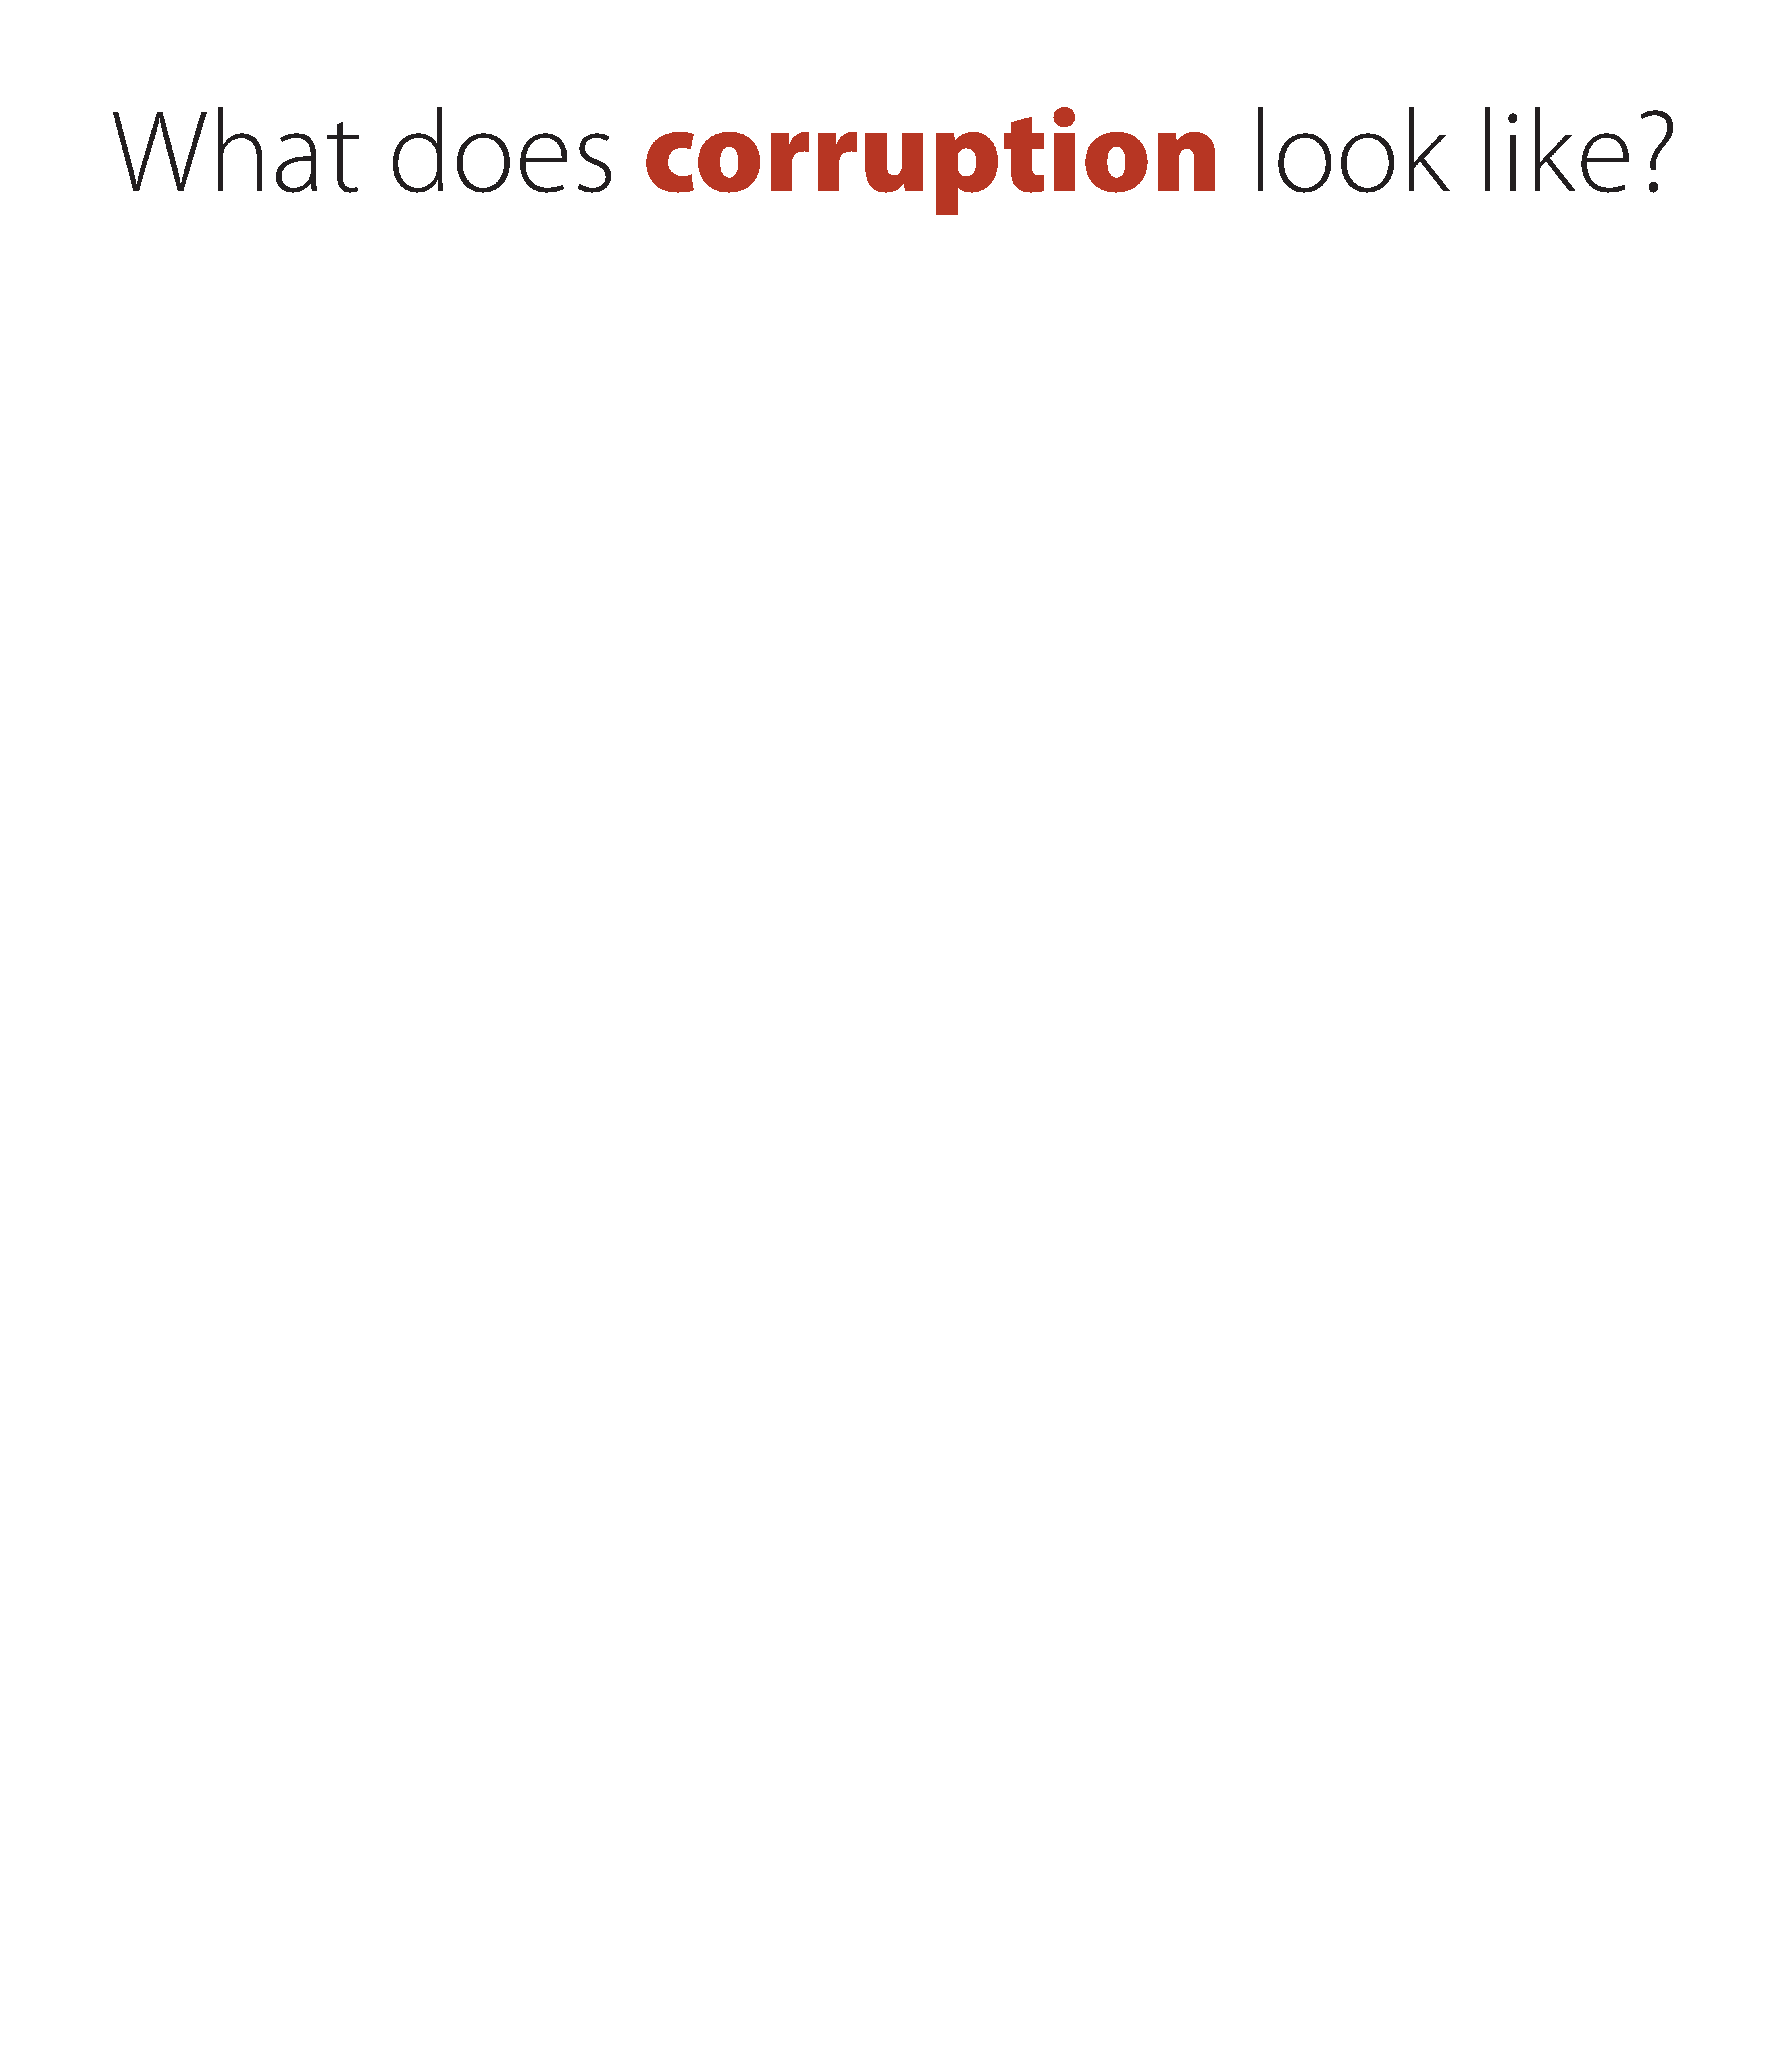
\includegraphics[max width=0.6\textwidth]{../img/poster_what.pdf}
\label{fig_what_corr}
\end{center}


\begin{subfigure}[t]{0.5\textwidth}
\caption{Cumulative value of non-competitive contracts}
\label{fig_cum_value}
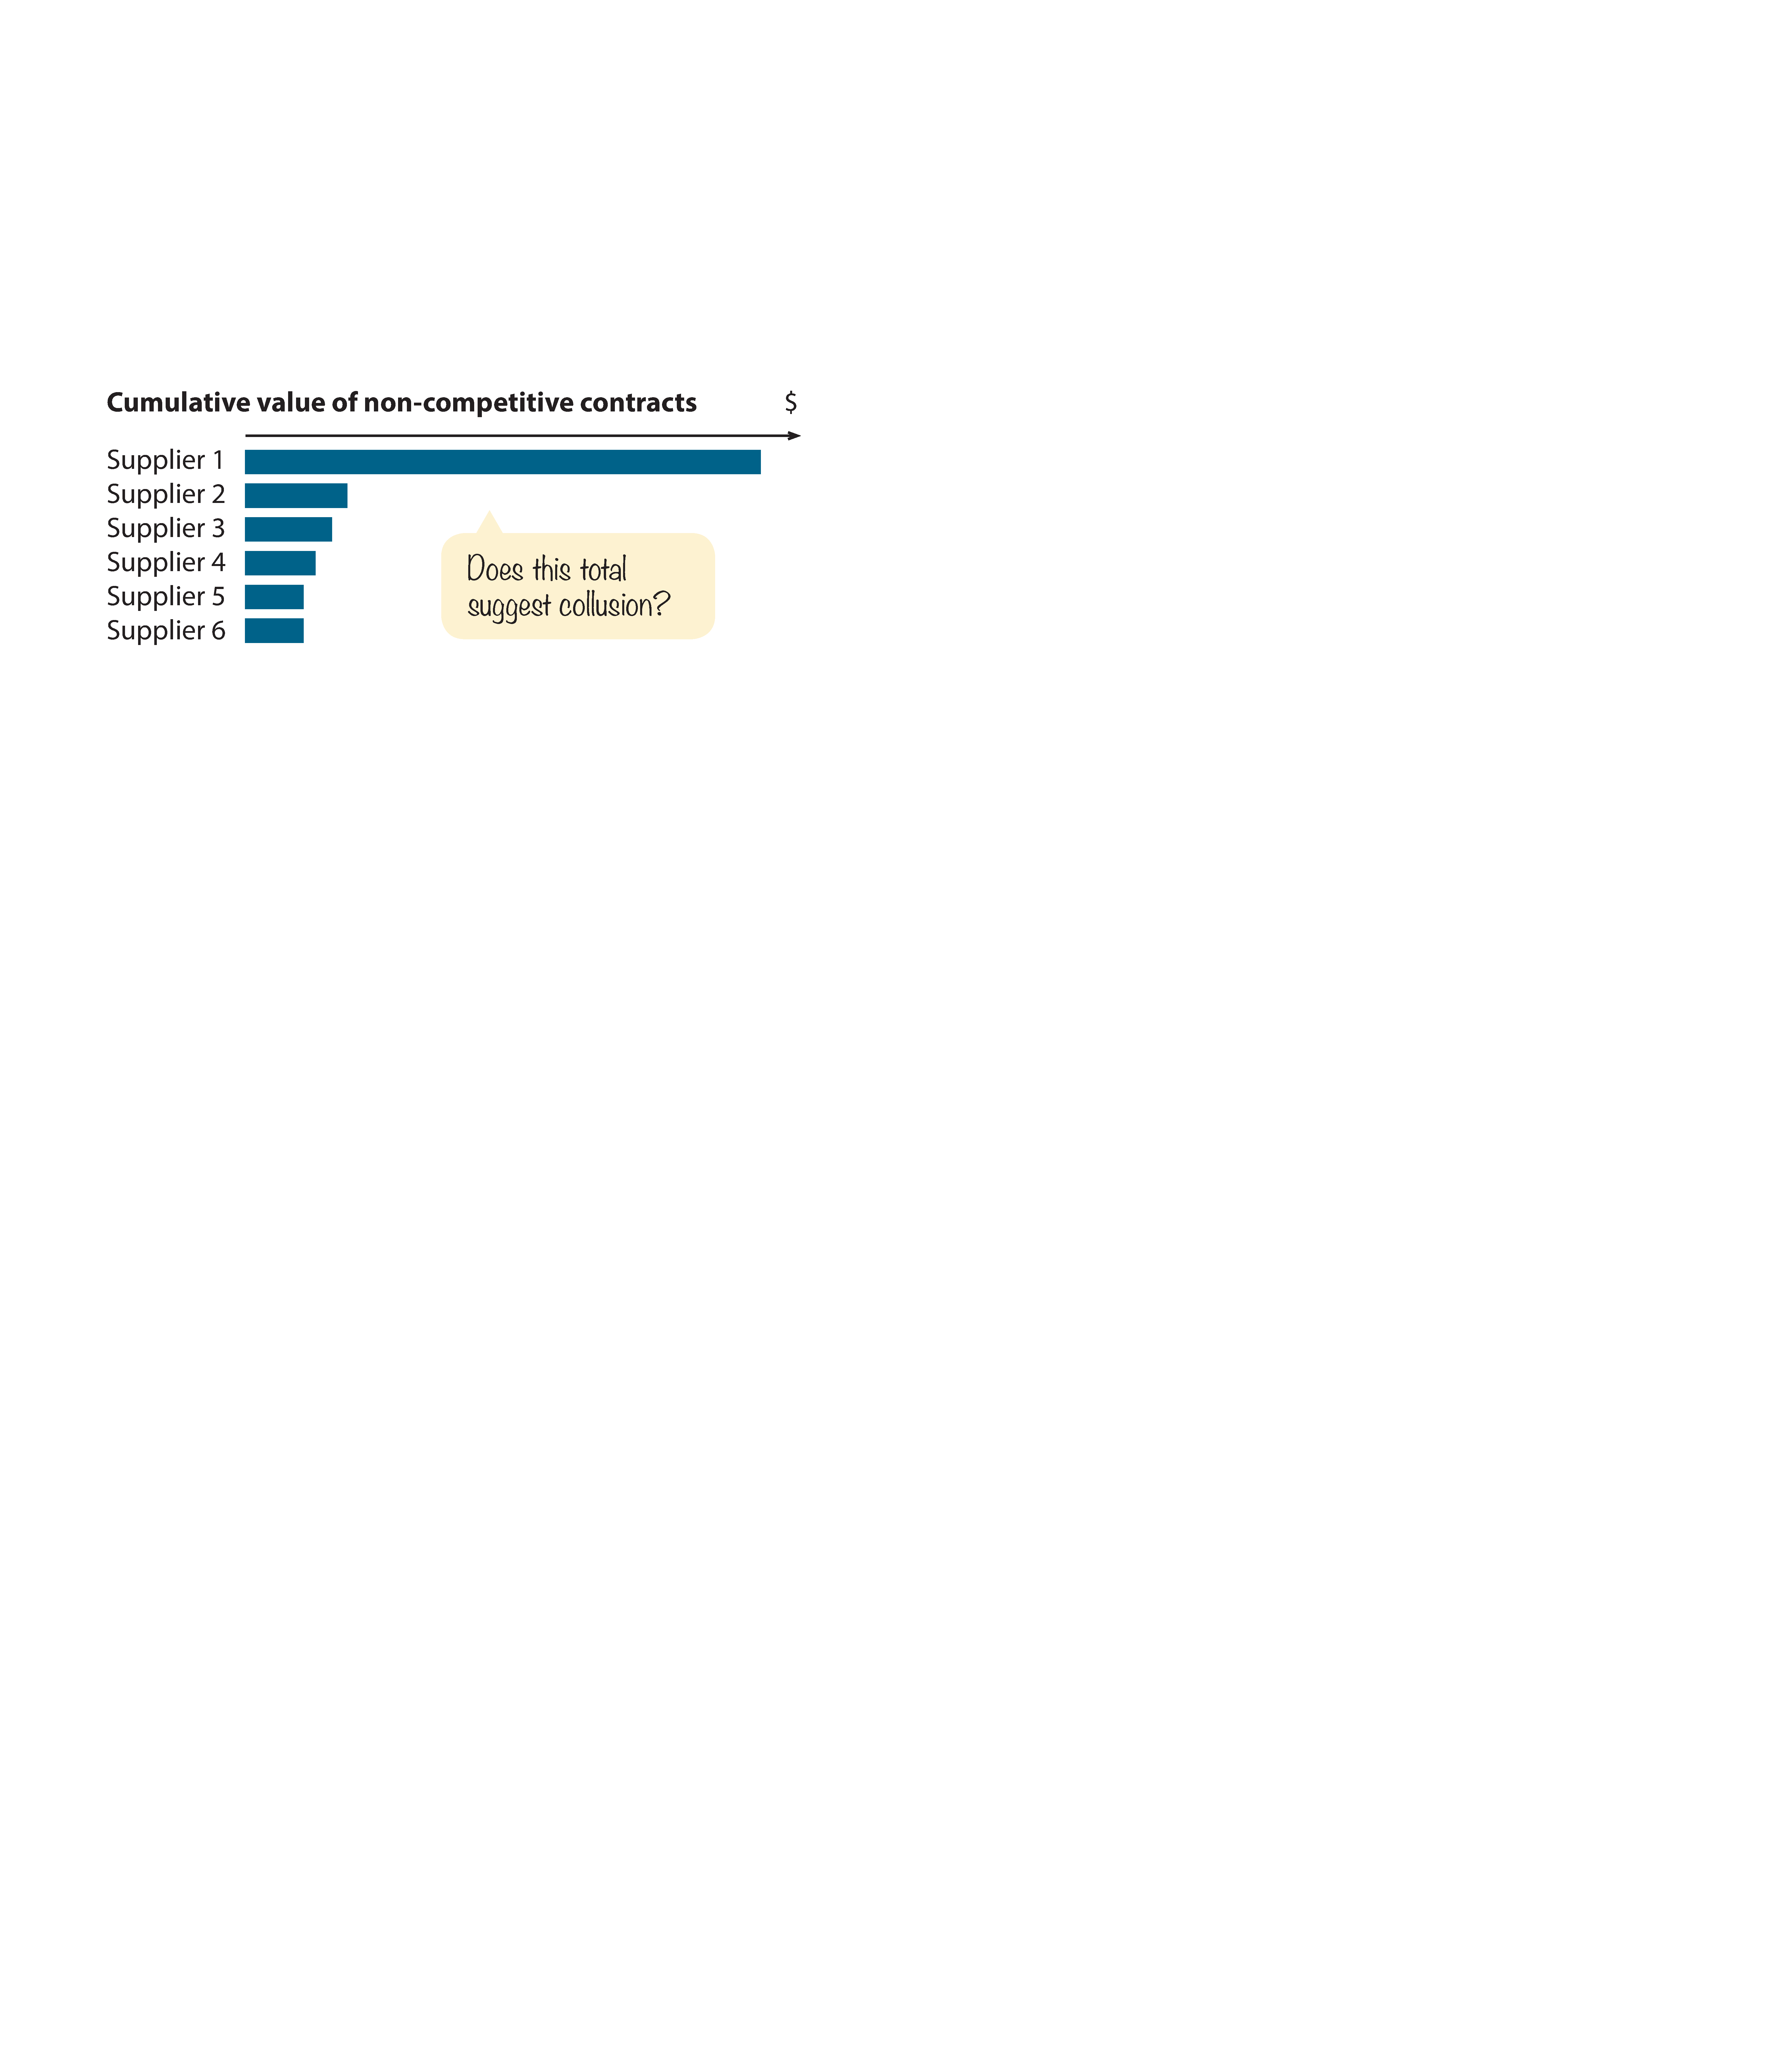
\includegraphics[max width=1\textwidth]{../img/poster_cumulative_value.pdf}
\end{subfigure}
~
\begin{subfigure}[t]{0.5\textwidth}
\caption{Value of Contracts}
\label{fig_value}
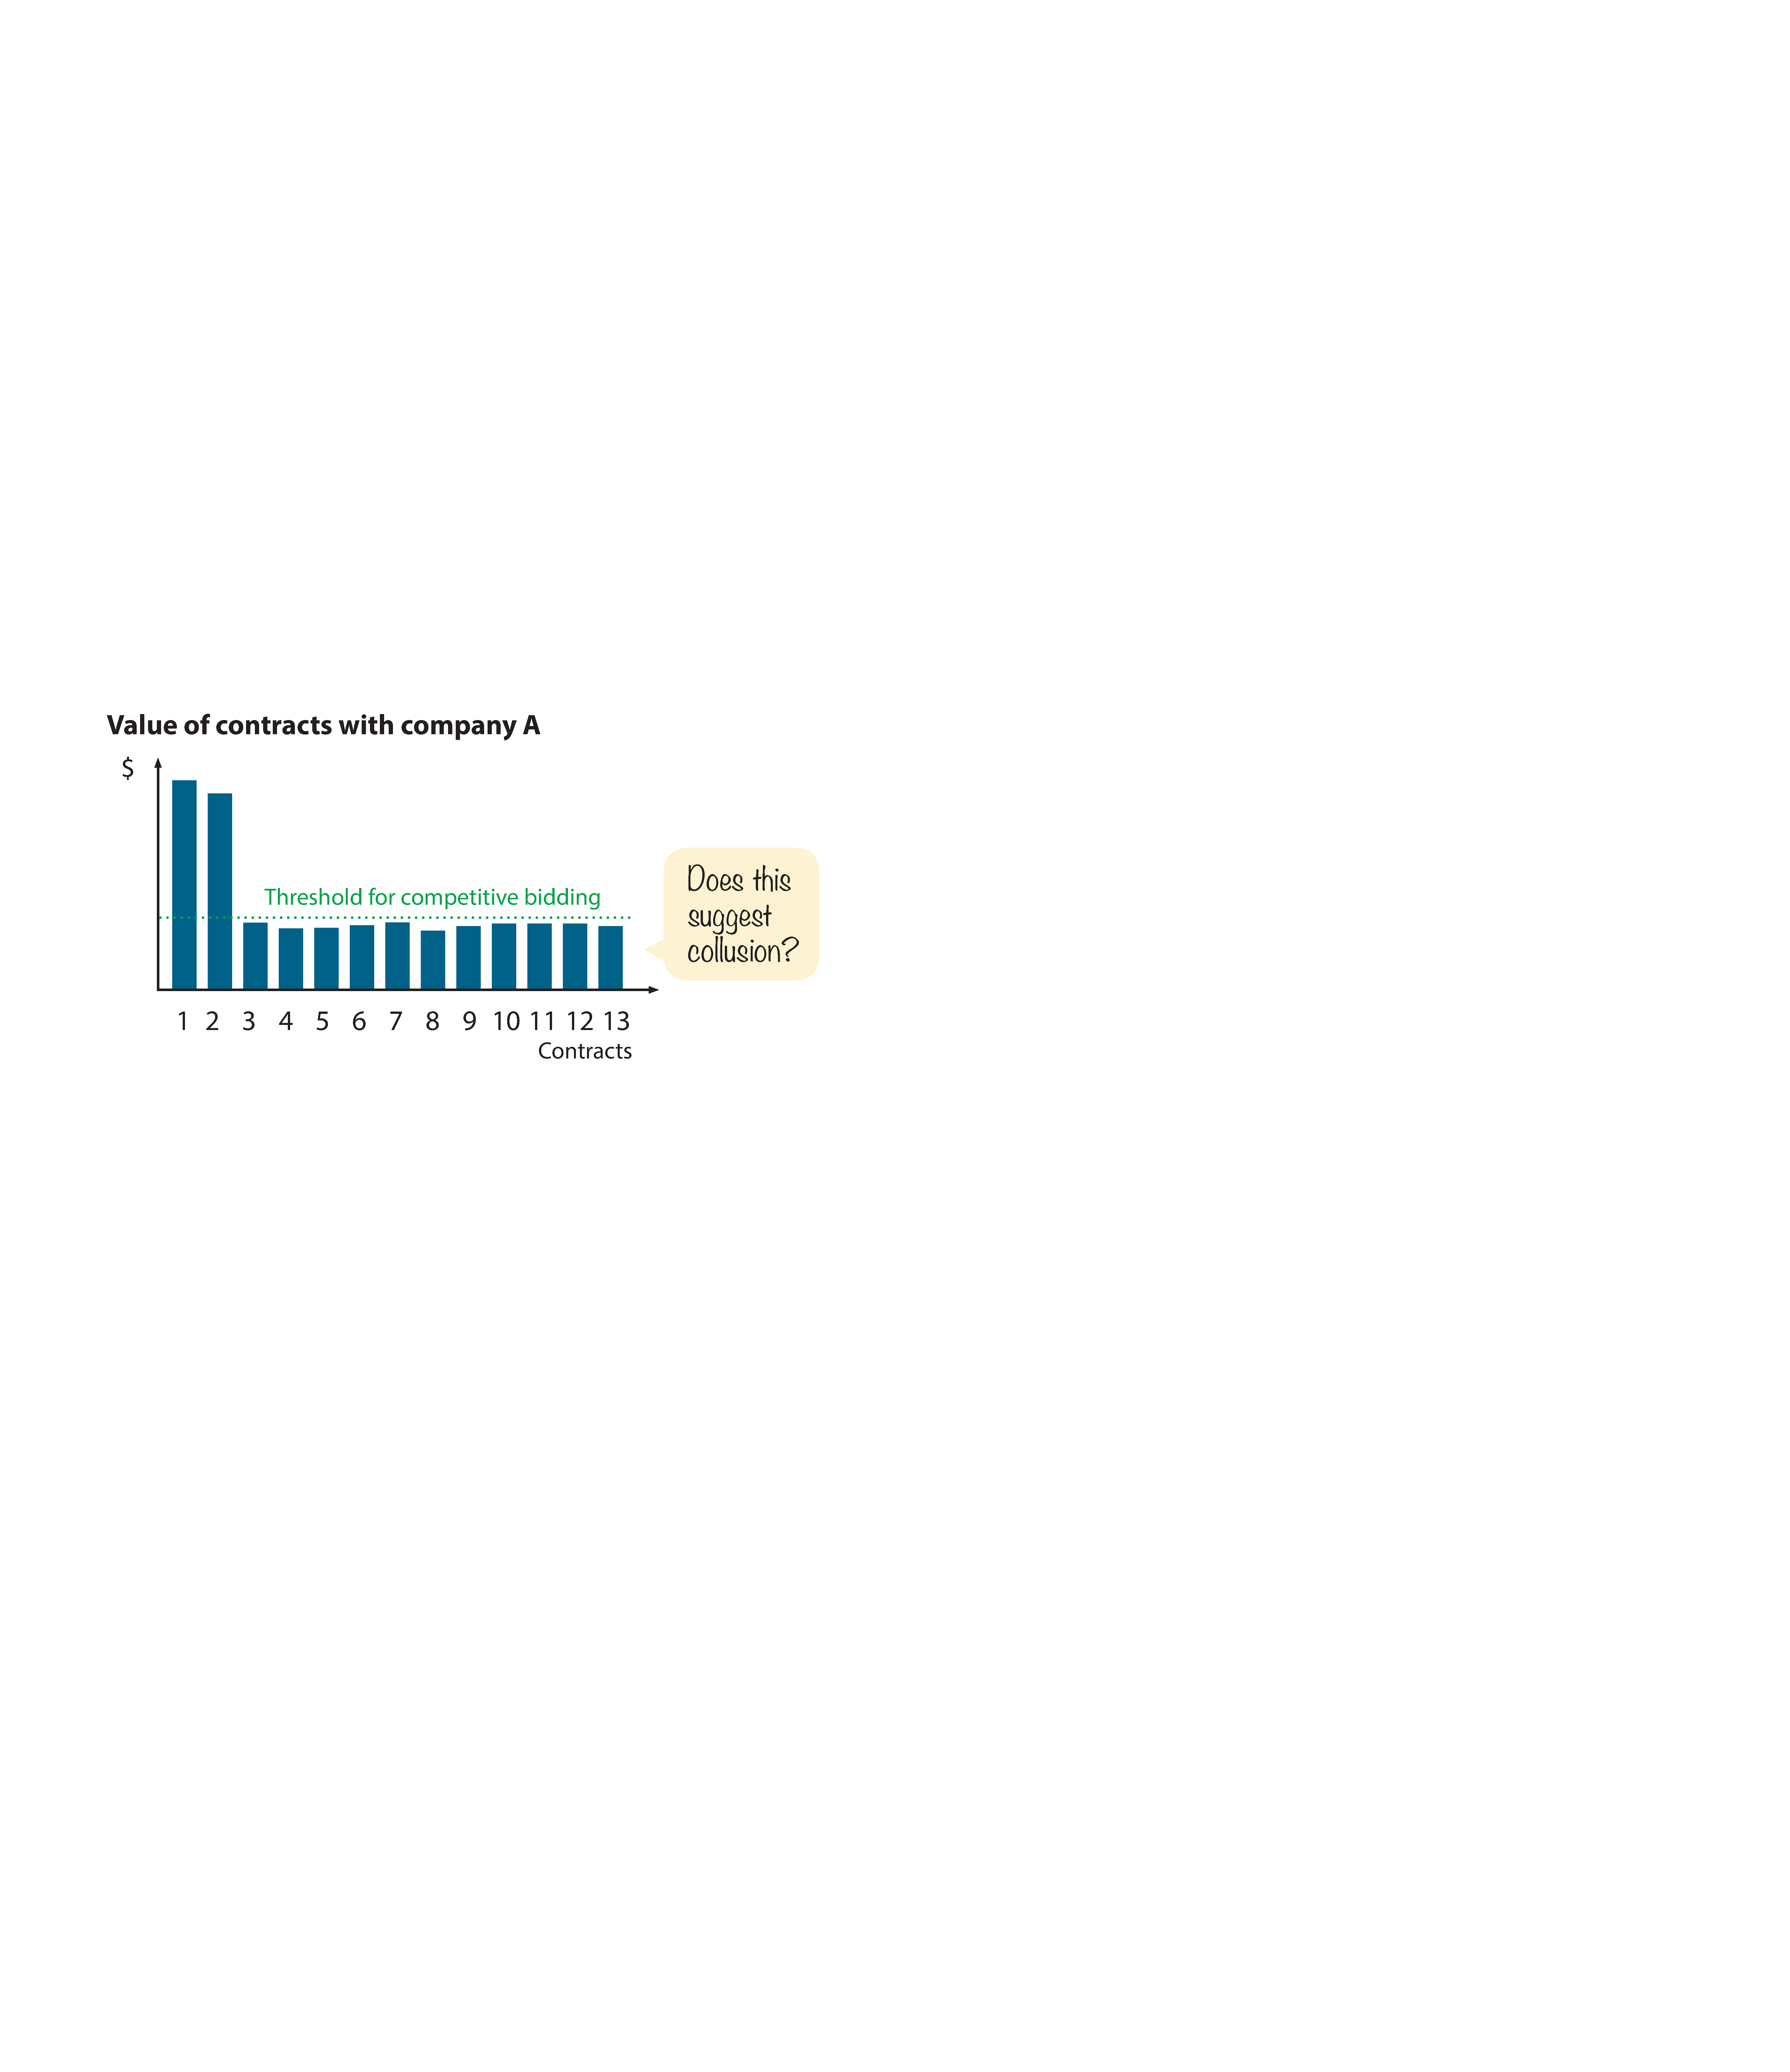
\includegraphics[max width=1\textwidth]{../img/poster_value.pdf}
\end{subfigure}
~
\begin{subfigure}[t]{0.5\textwidth}
\caption{Winning patterns}
\label{fig_winning}
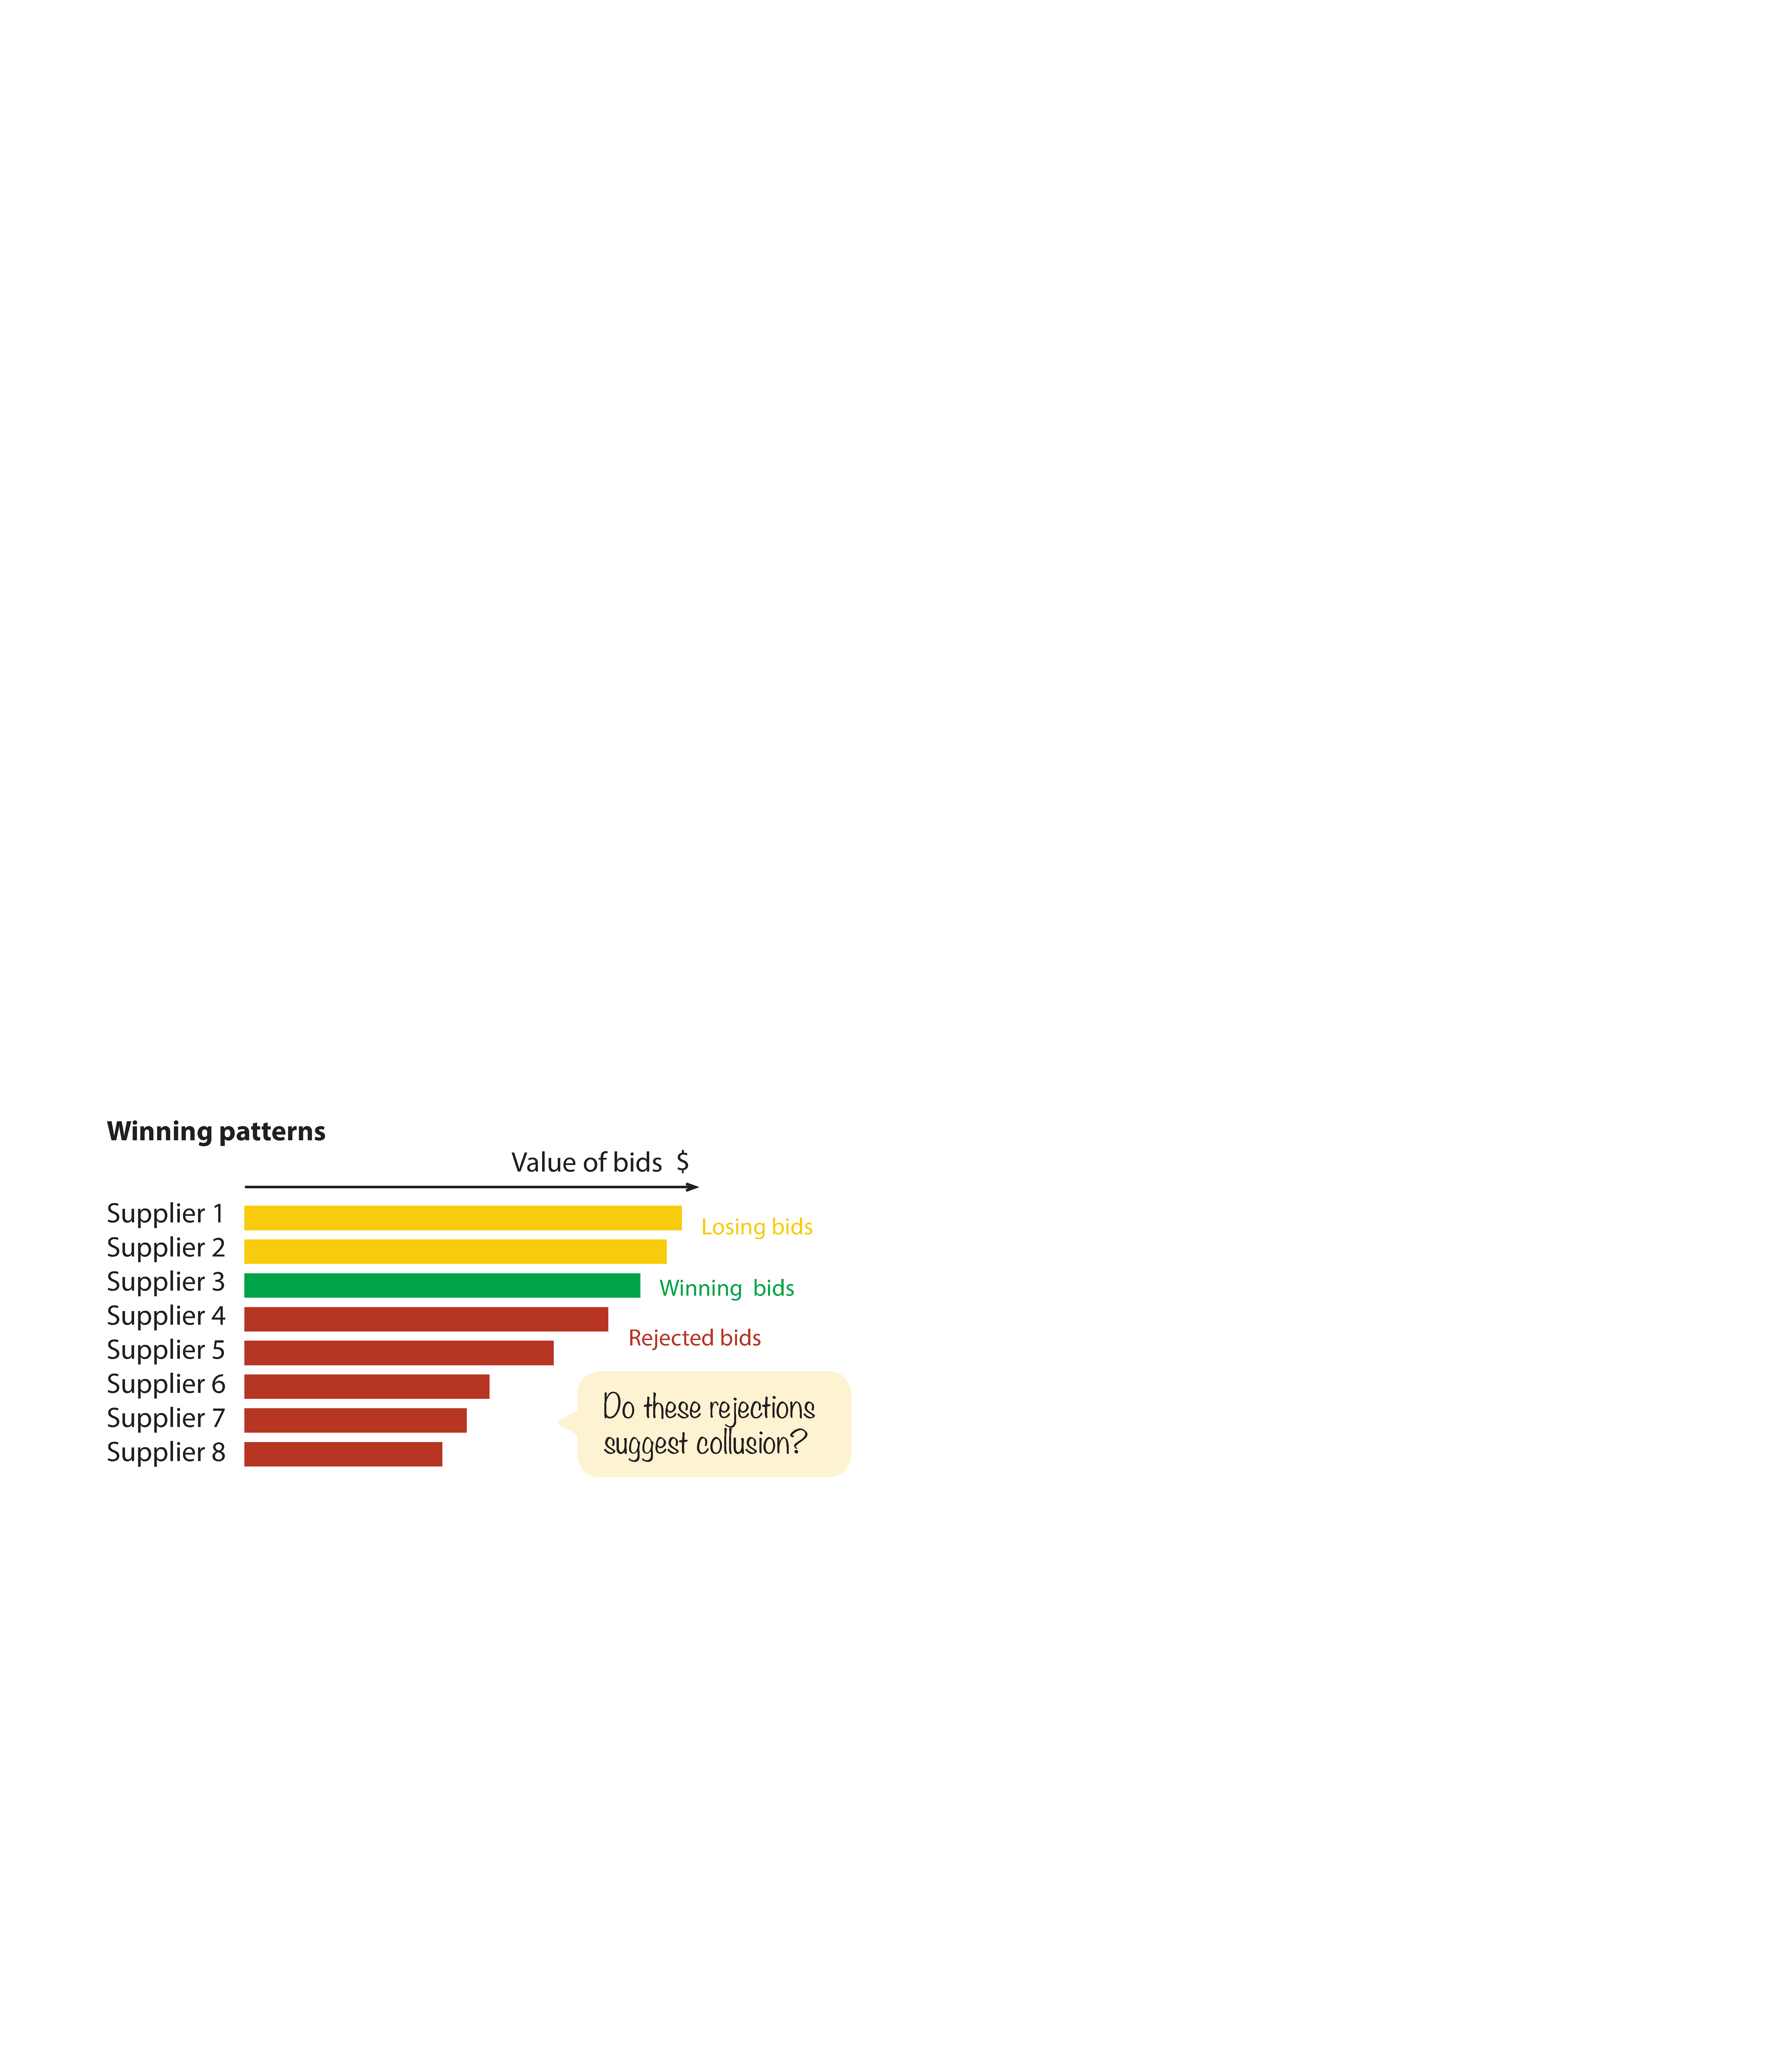
\includegraphics[max width=1\textwidth]{../img/poster_winning_patterns.pdf}
\end{subfigure}
~
\begin{subfigure}[t]{0.5\textwidth}
\caption{Monthly value of non-competitive contracts}
\label{fig_month}
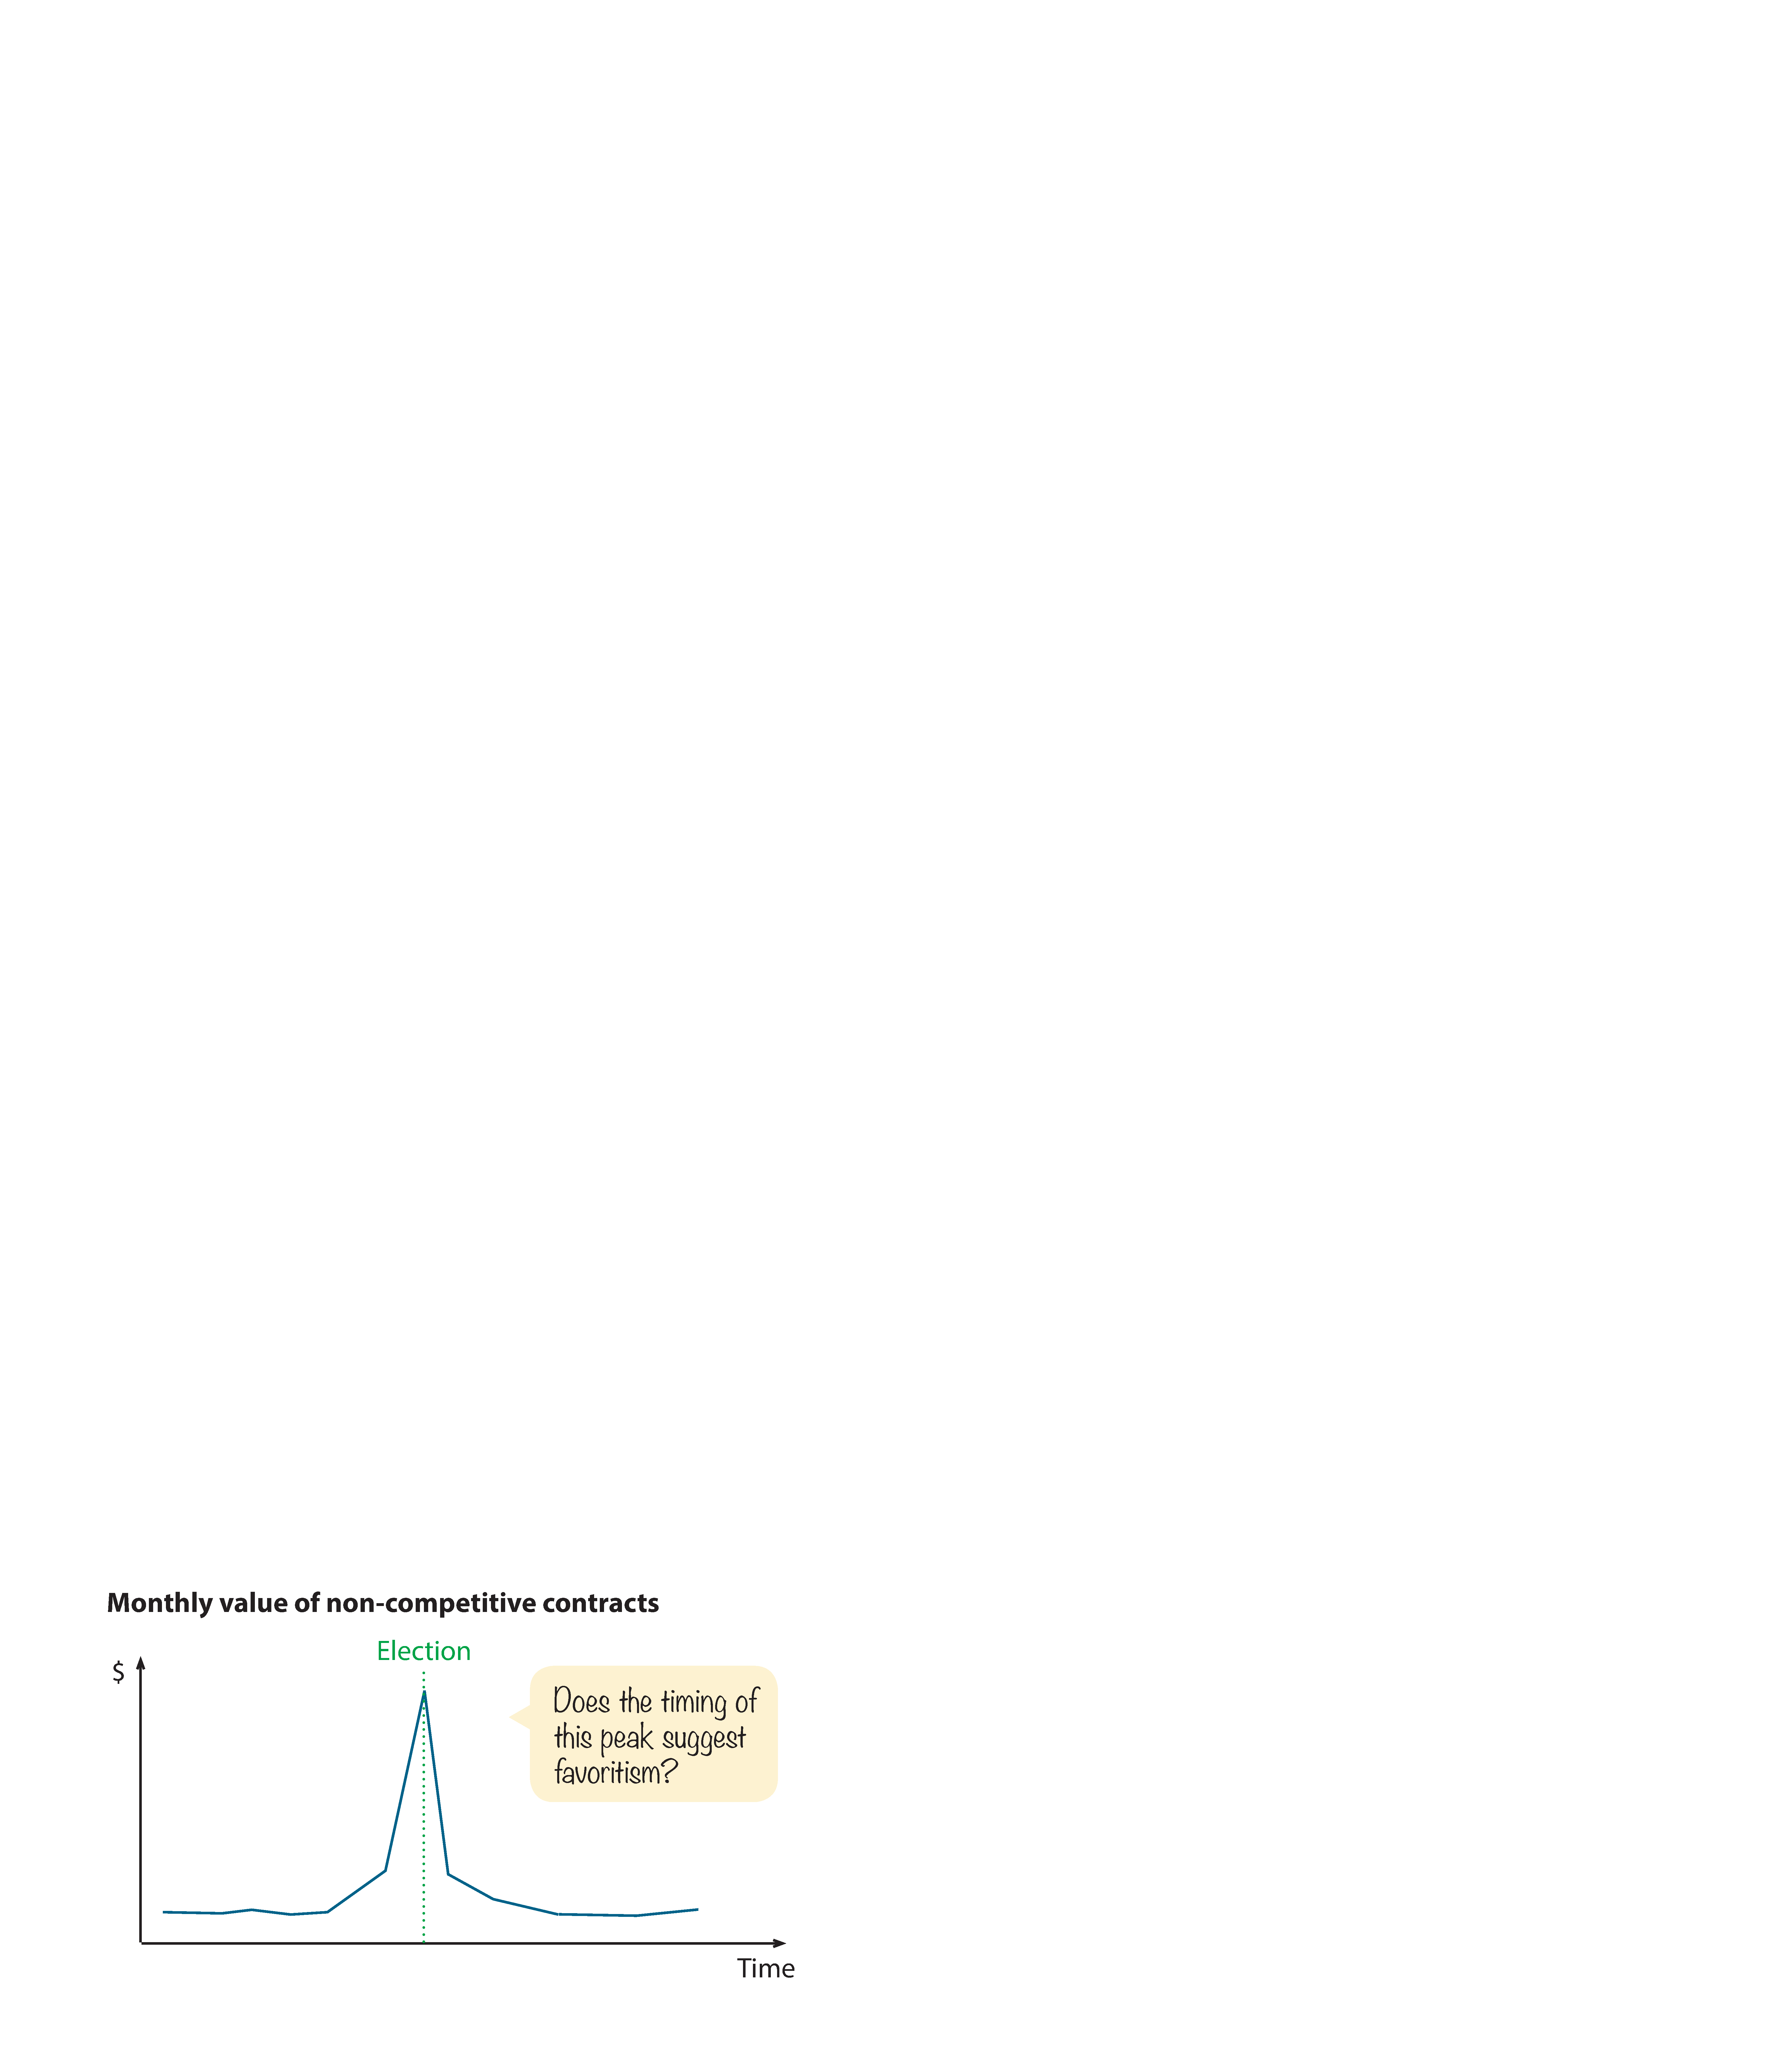
\includegraphics[max width=1\textwidth]{../img/poster_monthly.pdf}
\end{subfigure}
~
\begin{subfigure}[t]{0.5\textwidth}
\caption{Links between companies}
\label{fig_links}
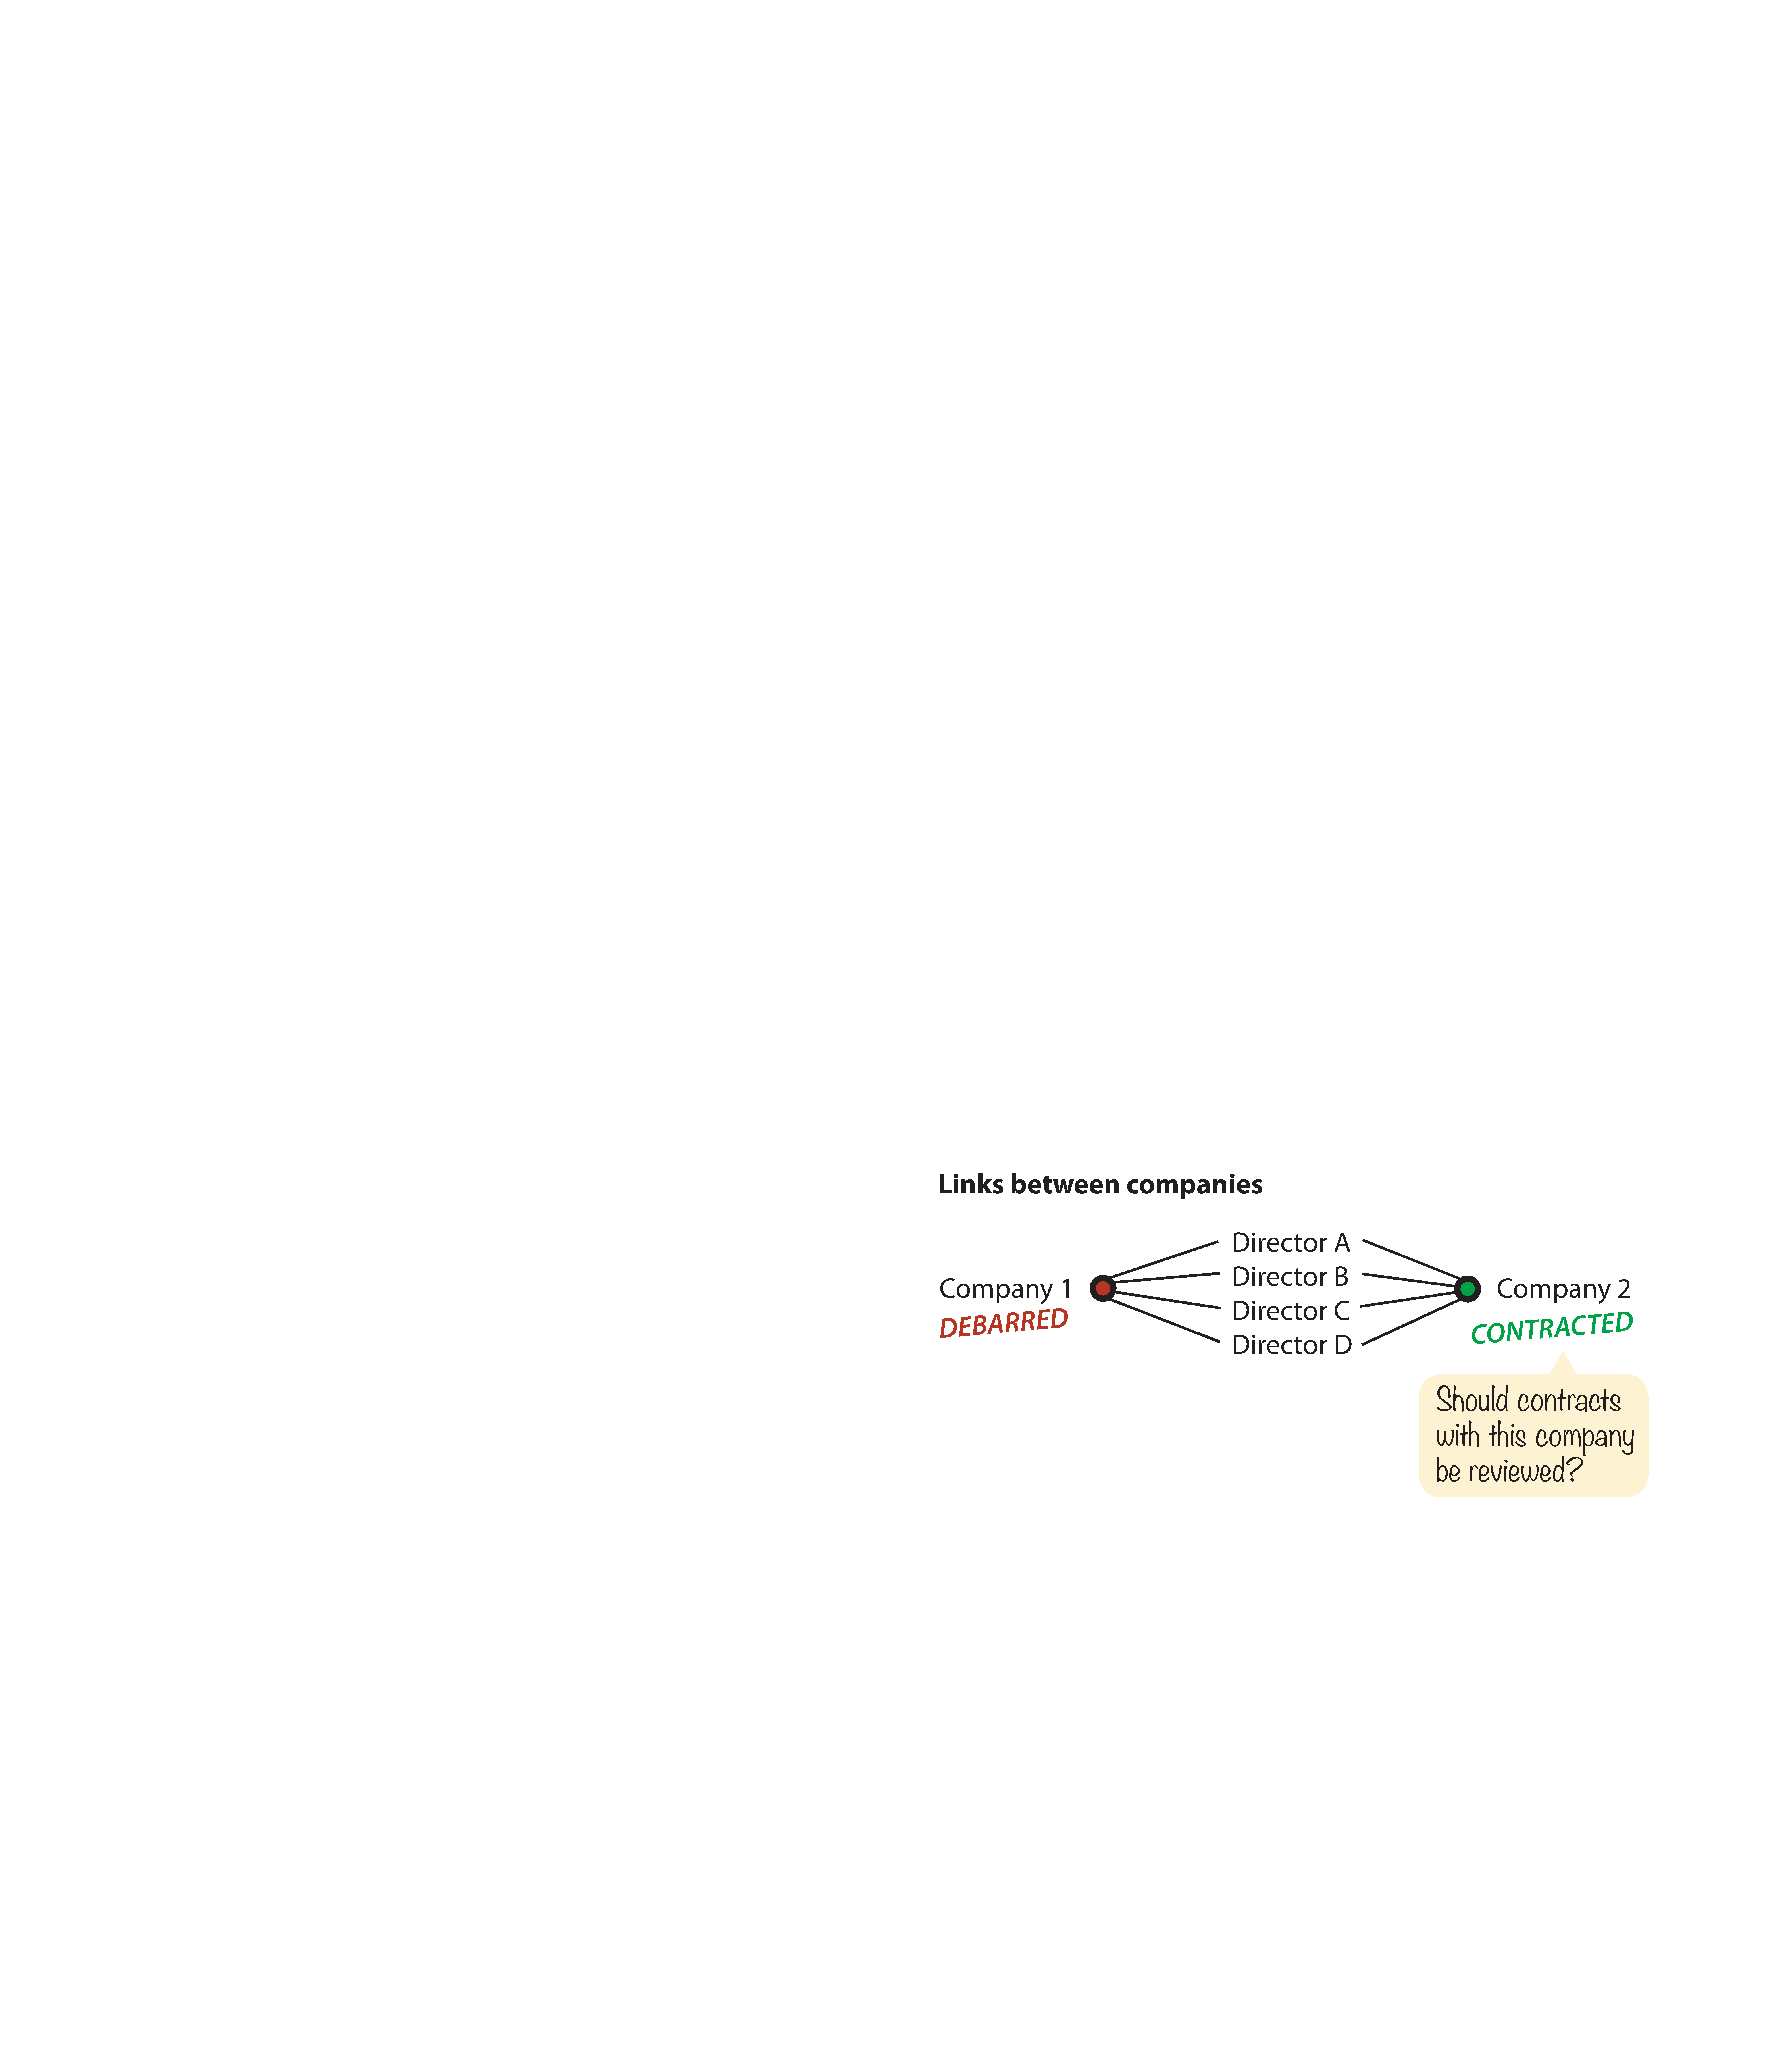
\includegraphics[max width=1\textwidth]{../img/poster_link.pdf}
\end{subfigure}
~
\begin{subfigure}[t]{0.5\textwidth}
\caption{Bidding patterns}
\label{fig_bid1}
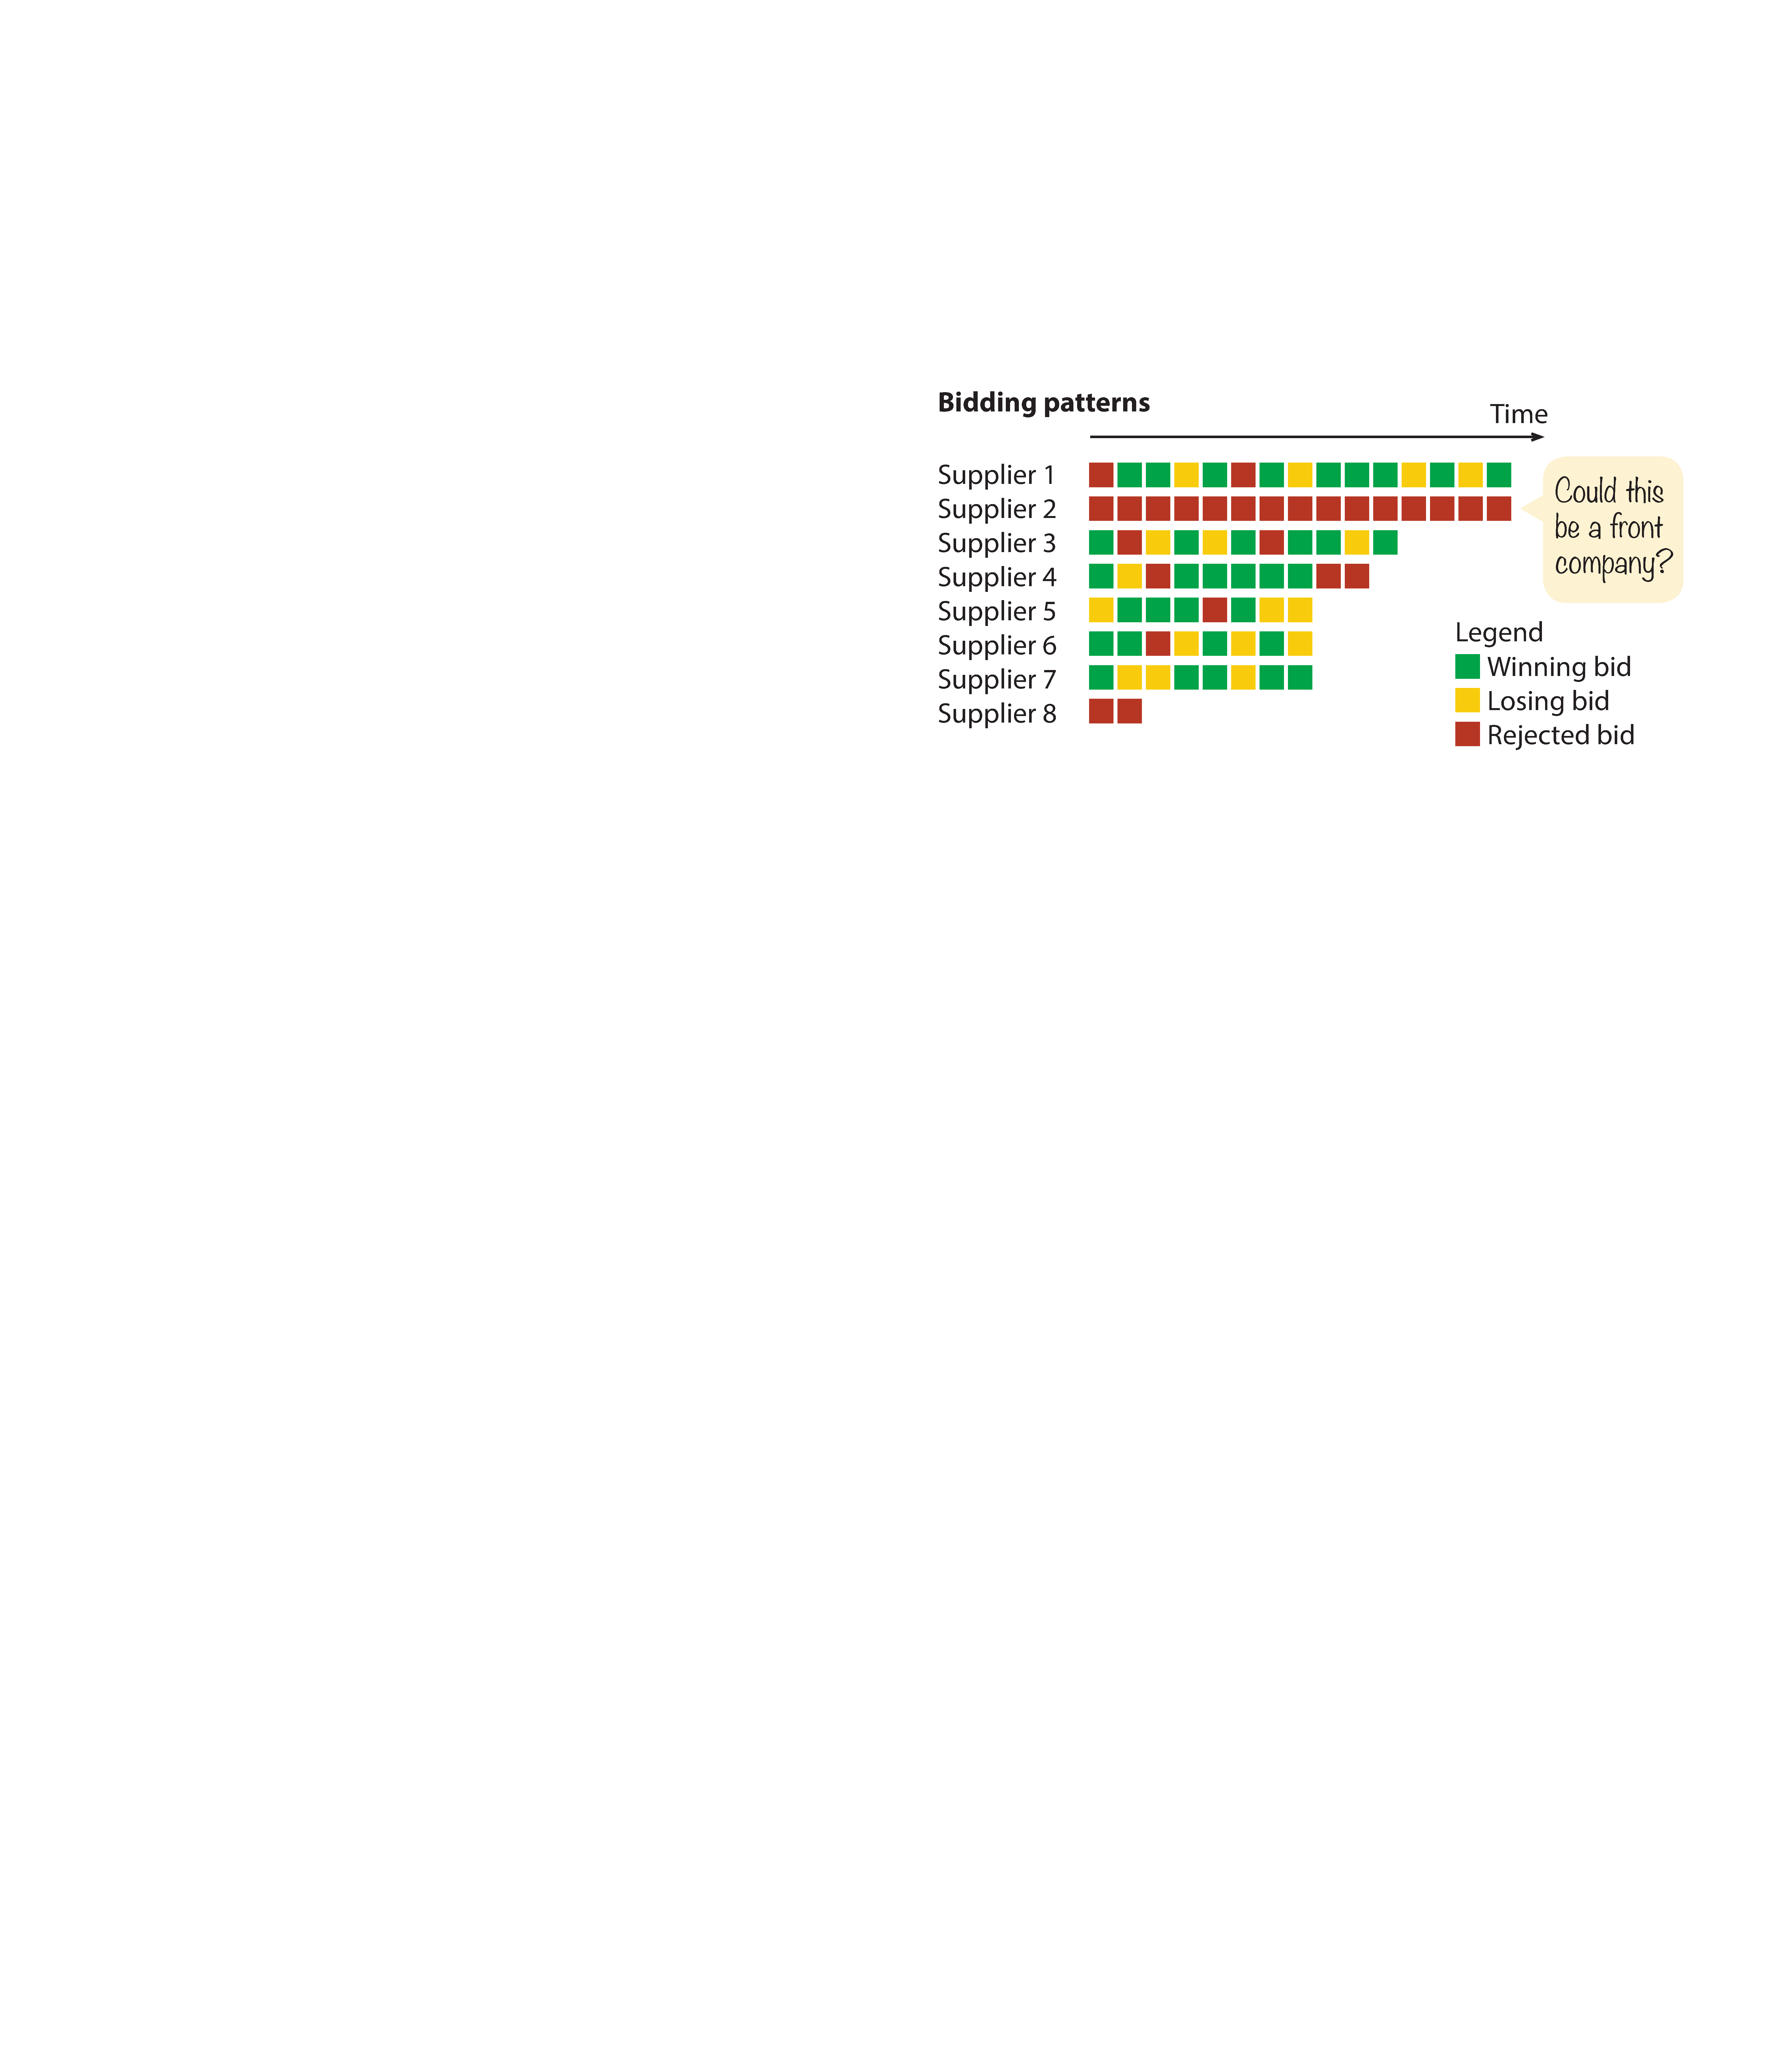
\includegraphics[max width=1\textwidth]{../img/poster_bidding_patt.pdf}
\end{subfigure}

\end{figure}
\clearpage
\begin{figure}[H]
\ContinuedFloat

\begin{subfigure}[t]{0.5\textwidth}
\caption{Participation to call for proposals}
\label{fig_proposals}
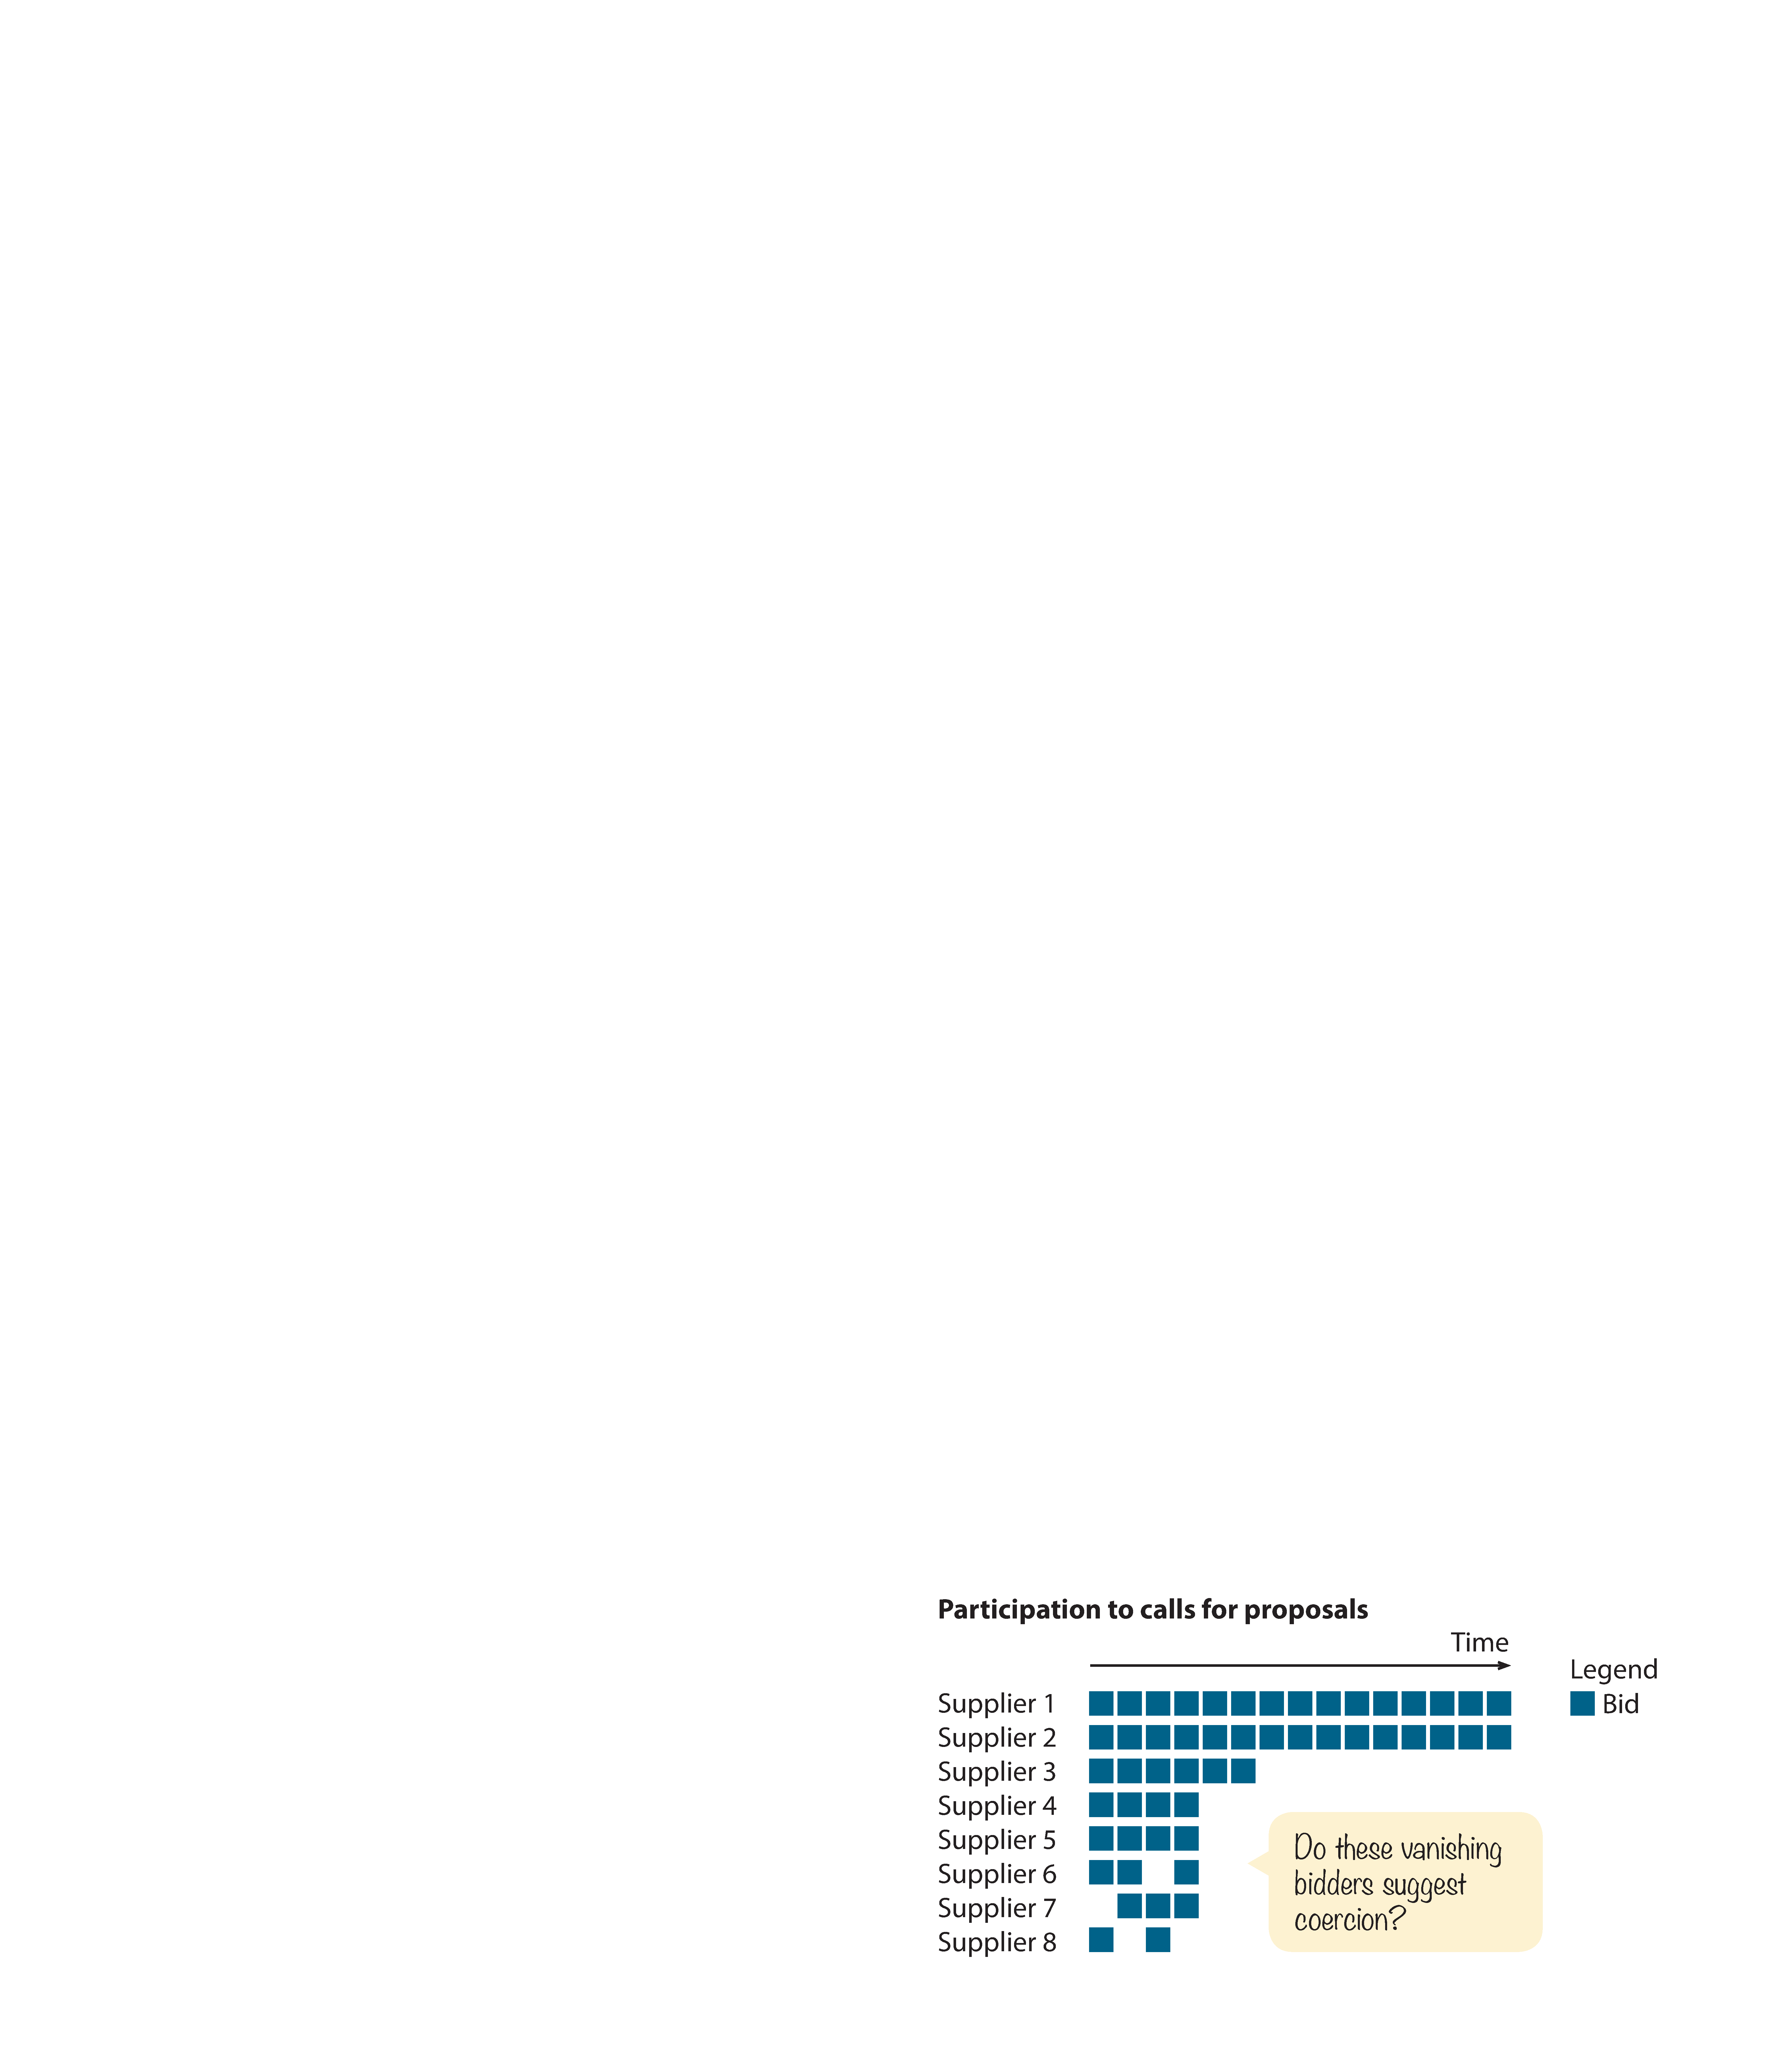
\includegraphics[max width=1\textwidth]{../img/poster_coercion.pdf}
\end{subfigure}
~
\begin{subfigure}[t]{0.5\textwidth}
\caption{Bidding patterns}
\label{fig_bid2}
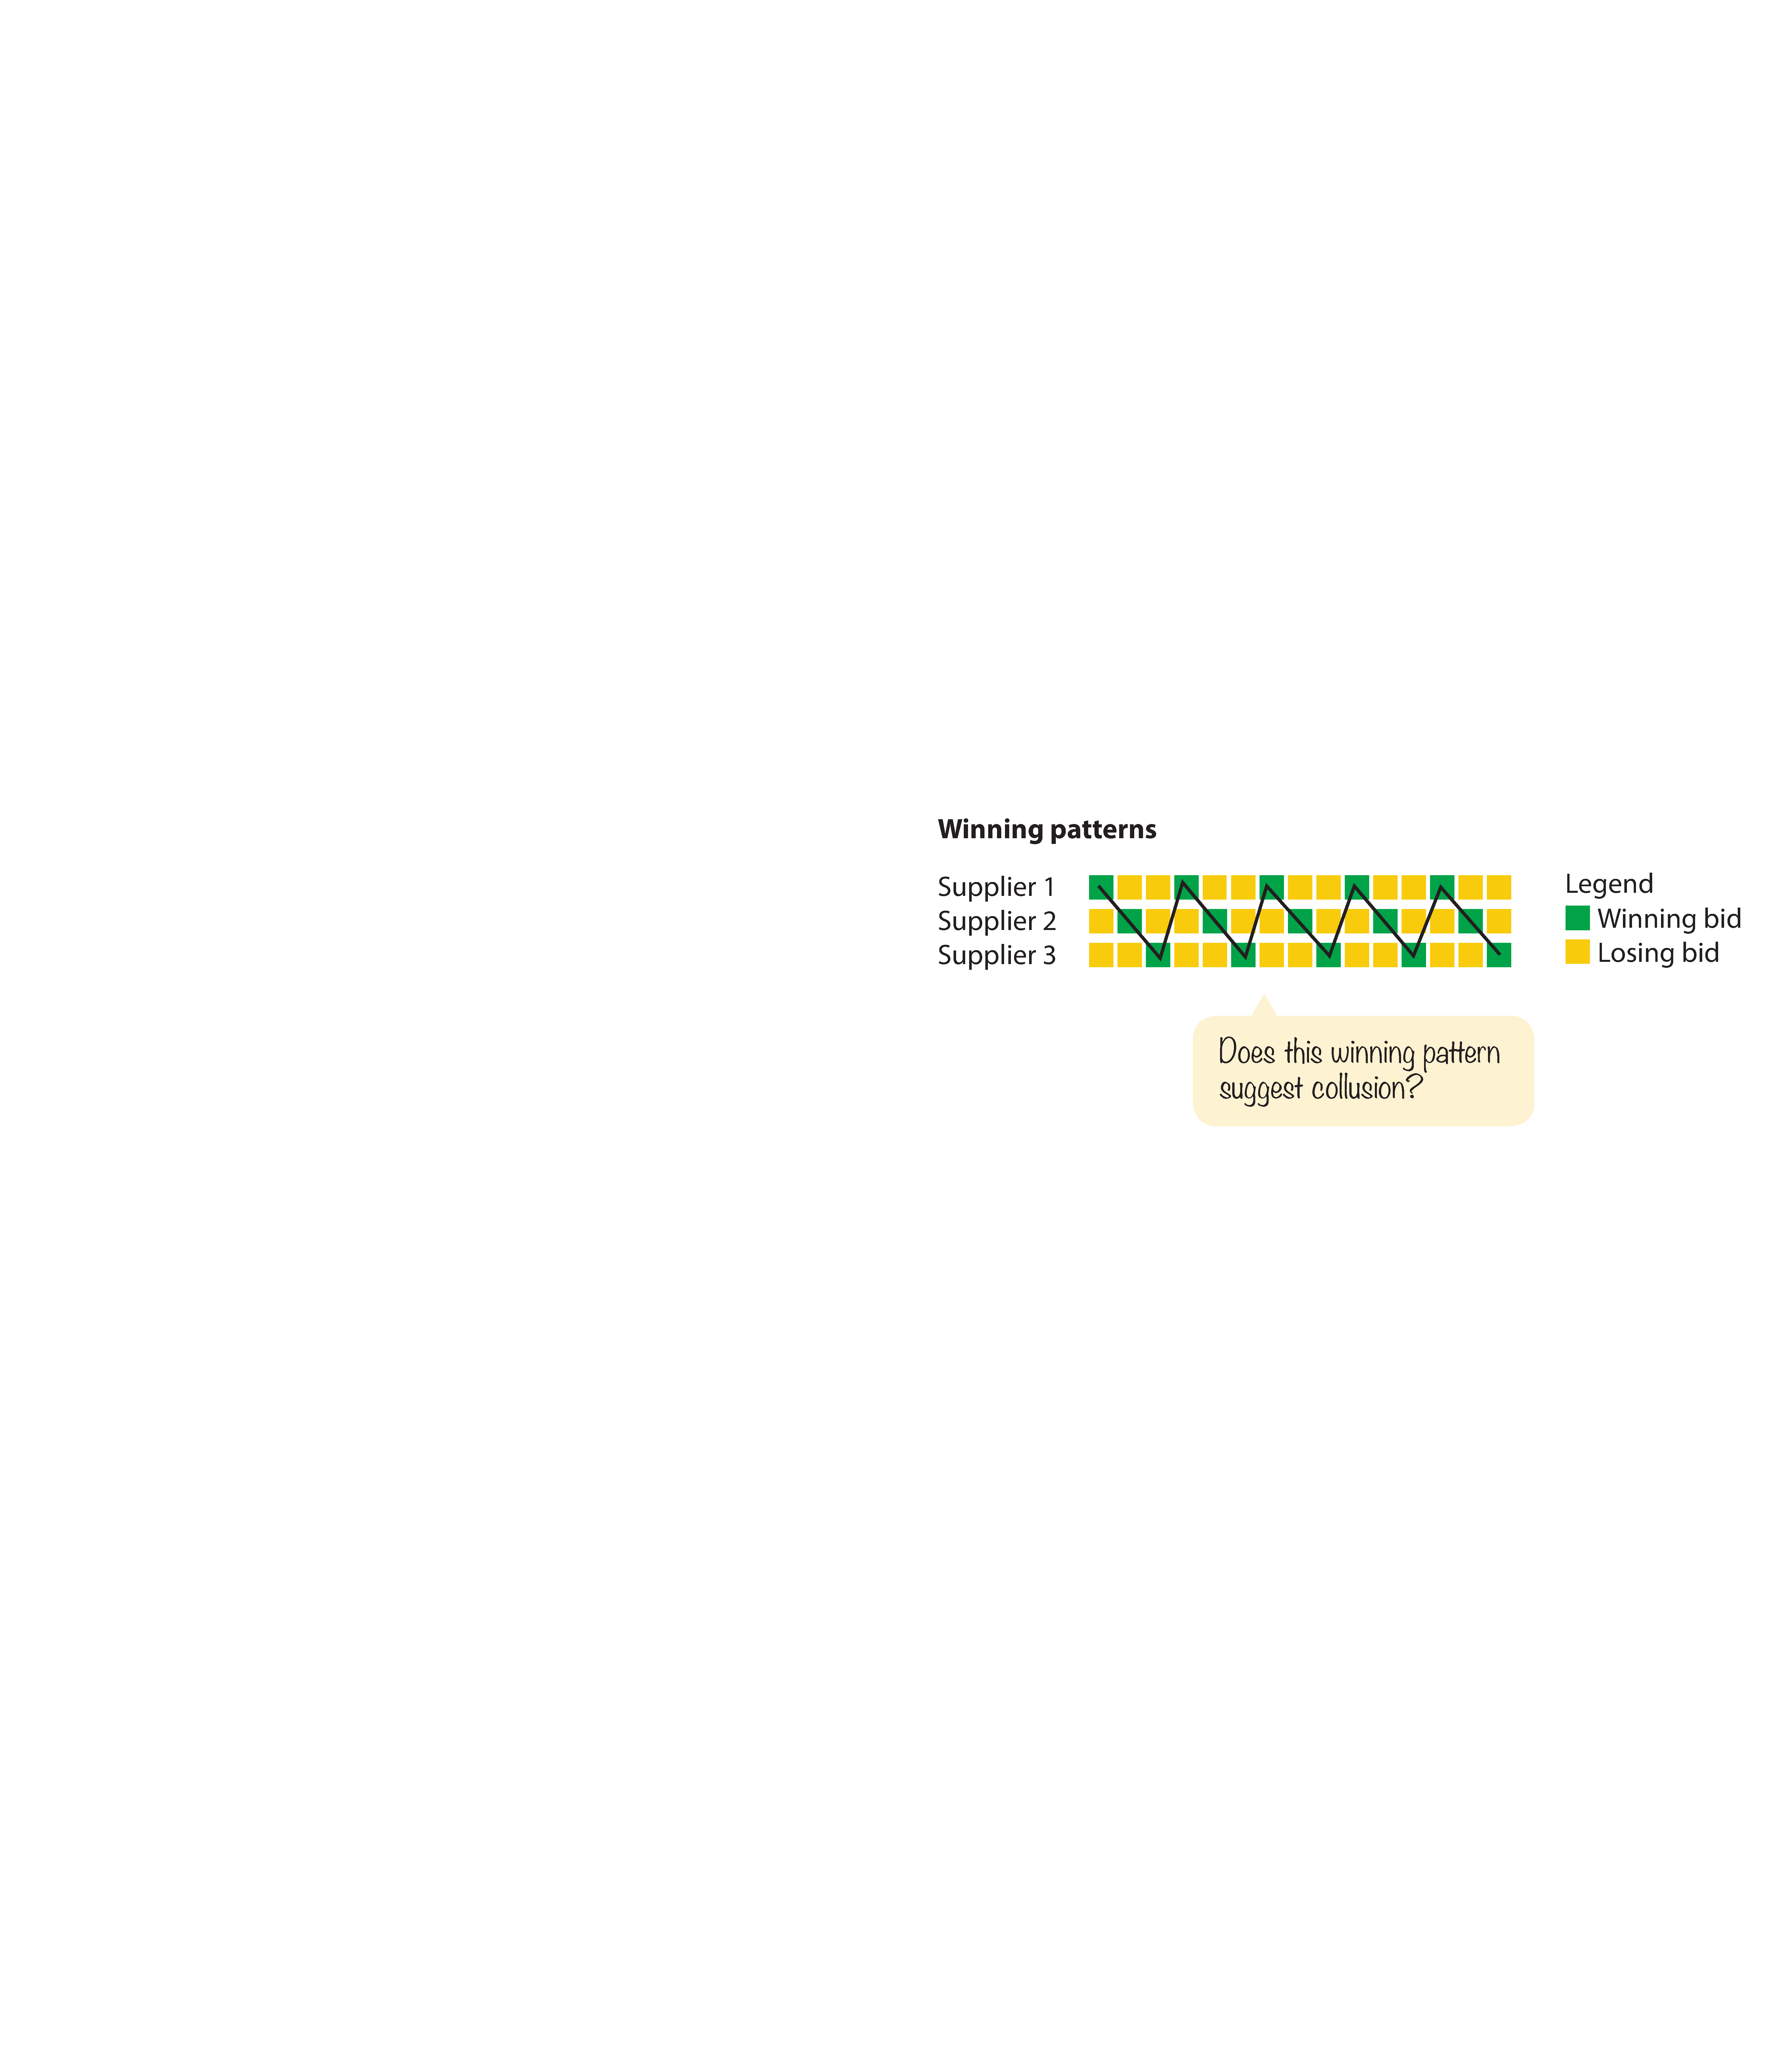
\includegraphics[max width=1\textwidth]{../img/poster_win_pattern.pdf}
\end{subfigure}
\footnotesize{\textbf{Source:} Figures taken from \cite{wb_poster}}
\end{figure}

Another priority during the trip to Washington D.C. was asking questions and learning about the data that will provide a window into the problems that INT is working to address. To data scientists, diving into analysis and model-building right away can be an enticing prospect when presented with an exciting new data set, but engaging with stakeholders and domain experts at the earliest stages can help guide analysis and save considerable time down the road.






